%-----------------------------------------------------------------------------------------
% Autor dieser Vorlage:
% Stefan Macke (http://fachinformatiker-anwendungsentwicklung.net)
% Permalink zur Vorlage: http://fiae.link/LaTeXVorlageFIAE
%
% Sämtliche verwendeten Abbildungen, Tabellen und Listings stammen von Dirk Grashorn.
%
% Lizenz: Creative Commons 4.0 Namensnennung - Weitergabe unter gleichen Bedingungen
% -----------------------------------------------------------------------------------------

\documentclass[
	ngerman,
	toc=listof, % Abbildungsverzeichnis sowie Tabellenverzeichnis in das Inhaltsverzeichnis aufnehmen
	toc=bibliography, % Literaturverzeichnis in das Inhaltsverzeichnis aufnehmen
	footnotes=multiple, % Trennen von direkt aufeinander folgenden Fußnoten
	parskip=half, % vertikalen Abstand zwischen Absätzen verwenden anstatt horizontale Einrückung von Folgeabsätzen
	numbers=noendperiod % Den letzten Punkt nach einer Nummerierung entfernen (nach DIN 5008)
]{scrartcl}
\pdfminorversion=5 % erlaubt das Einfügen von pdf-Dateien bis Version 1.7, ohne eine Fehlermeldung zu werfen (keine Garantie für fehlerfreies Einbetten!)
\usepackage[utf8]{inputenc} % muss als erstes eingebunden werden, da Meta/Packages ggfs. Sonderzeichen enthalten

% !TEX root = Projektdokumentation.tex

% Hinweis: der Titel muss zum Inhalt des Projekts passen und den zentralen Inhalt des Projekts deutlich herausstellen
\newcommand{\titel}{Entwicklung von NatInfo}
\newcommand{\untertitel}{Webbasiertes Tool zur Unterstützung der Entwickler}
\newcommand{\kompletterTitel}{\titel{} -- \untertitel}

\newcommand{\autorName}{Stefan Macke}
\newcommand{\autorAnschrift}{Meine Straße 1}
\newcommand{\autorOrt}{49377 Vechta}

\newcommand{\betriebLogo}{LogoBetrieb.pdf}
\newcommand{\betriebName}{\textsc{Alte Oldenburger} Krankenversicherung AG}
\newcommand{\betriebAnschrift}{Theodor-Heuss-Str. 96}
\newcommand{\betriebOrt}{49377 Vechta}

\newcommand{\ausbildungsberuf}{Fachinformatiker für Anwendungsentwicklung}
\newcommand{\betreff}{Dokumentation zur betrieblichen Projektarbeit}
\newcommand{\pruefungstermin}{Sommer 2015}
\newcommand{\abgabeOrt}{Vechta}
\newcommand{\abgabeTermin}{23.04.2015}
 % Metadaten zu diesem Dokument (Autor usw.)
% !TEX root = ../Projektdokumentation.tex

% Anpassung an Landessprache ---------------------------------------------------
\usepackage{babel}

% Umlaute ----------------------------------------------------------------------
%   Umlaute/Sonderzeichen wie äüöß direkt im Quelltext verwenden (CodePage).
%   Erlaubt automatische Trennung von Worten mit Umlauten.
% ------------------------------------------------------------------------------
\usepackage[T1]{fontenc}
\usepackage{textcomp} % Euro-Zeichen etc.

% Schrift ----------------------------------------------------------------------
\usepackage{lmodern} % bessere Fonts
\usepackage{relsize} % Schriftgröße relativ festlegen

% Tabellen ---------------------------------------------------------------------
\PassOptionsToPackage{table}{xcolor}
\usepackage{tabularx}
% für lange Tabellen
\usepackage{longtable}
\usepackage{array}
\usepackage{ragged2e}
\usepackage{lscape}
\newcolumntype{w}[1]{>{\raggedleft\hspace{0pt}}p{#1}} % Spaltendefinition rechtsbündig mit definierter Breite

% Grafiken ---------------------------------------------------------------------
\usepackage[dvips,final]{graphicx} % Einbinden von JPG-Grafiken ermöglichen
\usepackage{graphics} % keepaspectratio
\usepackage{floatflt} % zum Umfließen von Bildern
\graphicspath{{Bilder/}} % hier liegen die Bilder des Dokuments

% Sonstiges --------------------------------------------------------------------
\usepackage[titles]{tocloft} % Inhaltsverzeichnis DIN 5008 gerecht einrücken
\usepackage{amsmath,amsfonts} % Befehle aus AMSTeX für mathematische Symbole
\usepackage{enumitem} % anpassbare Enumerates/Itemizes
\usepackage{xspace} % sorgt dafür, dass Leerzeichen hinter parameterlosen Makros nicht als Makroendezeichen interpretiert werden

\usepackage{makeidx} % für Index-Ausgabe mit \printindex
\usepackage[printonlyused]{acronym} % es werden nur benutzte Definitionen aufgelistet

% Einfache Definition der Zeilenabstände und Seitenränder etc.
\usepackage{setspace}
\usepackage{geometry}

% Symbolverzeichnis
\usepackage[intoc]{nomencl}
\let\abbrev\nomenclature
\renewcommand{\nomname}{Abkürzungsverzeichnis}
\setlength{\nomlabelwidth}{.25\hsize}
\renewcommand{\nomlabel}[1]{#1 \dotfill}
\setlength{\nomitemsep}{-\parsep}

\usepackage{varioref} % Elegantere Verweise. „auf der nächsten Seite“
\usepackage{url} % URL verlinken, lange URLs umbrechen etc.

\usepackage{chngcntr} % fortlaufendes Durchnummerieren der Fußnoten
% \usepackage[perpage]{footmisc} % Alternative: Nummerierung der Fußnoten auf jeder Seite neu

\usepackage{ifthen} % bei der Definition eigener Befehle benötigt
\usepackage{todonotes} % definiert u.a. die Befehle \todo und \listoftodos
\usepackage[square]{natbib} % wichtig für korrekte Zitierweise

% PDF-Optionen -----------------------------------------------------------------
\usepackage{pdfpages}
\pdfminorversion=5 % erlaubt das Einfügen von pdf-Dateien bis Version 1.7, ohne eine Fehlermeldung zu werfen (keine Garantie für fehlerfreies Einbetten!)
\usepackage[
    bookmarks,
    bookmarksnumbered,
    bookmarksopen=true,
    bookmarksopenlevel=1,
    colorlinks=true,
% diese Farbdefinitionen zeichnen Links im PDF farblich aus
    linkcolor=AOBlau, % einfache interne Verknüpfungen
    anchorcolor=AOBlau,% Ankertext
    citecolor=AOBlau, % Verweise auf Literaturverzeichniseinträge im Text
    filecolor=AOBlau, % Verknüpfungen, die lokale Dateien öffnen
    menucolor=AOBlau, % Acrobat-Menüpunkte
    urlcolor=AOBlau,
% diese Farbdefinitionen sollten für den Druck verwendet werden (alles schwarz)
    %linkcolor=black, % einfache interne Verknüpfungen
    %anchorcolor=black, % Ankertext
    %citecolor=black, % Verweise auf Literaturverzeichniseinträge im Text
    %filecolor=black, % Verknüpfungen, die lokale Dateien öffnen
    %menucolor=black, % Acrobat-Menüpunkte
    %urlcolor=black,
%
    %backref, % Quellen werden zurück auf ihre Zitate verlinkt
    pdftex,
    plainpages=false, % zur korrekten Erstellung der Bookmarks
    pdfpagelabels=true, % zur korrekten Erstellung der Bookmarks
    hypertexnames=false, % zur korrekten Erstellung der Bookmarks
    linktocpage % Seitenzahlen anstatt Text im Inhaltsverzeichnis verlinken
]{hyperref}
% Befehle, die Umlaute ausgeben, führen zu Fehlern, wenn sie hyperref als Optionen übergeben werden
\hypersetup{
    pdftitle={\titel -- \untertitel},
    pdfauthor={\autorNameOne -- \autorNameTwo},
    pdfcreator={\autorNameOne -- \autorNameTwo},
    pdfsubject={\titel -- \untertitel},
    pdfkeywords={\titel -- \untertitel},
}


% zum Einbinden von Programmcode -----------------------------------------------
\usepackage{listings}
\usepackage{xcolor}
\definecolor{hellgelb}{rgb}{1,1,0.9}
\definecolor{colKeys}{rgb}{0,0,1}
\definecolor{colIdentifier}{rgb}{0,0,0}
\definecolor{colComments}{rgb}{0,0.5,0}
\definecolor{colString}{rgb}{1,0,0}
\lstset{
    float=hbp,
	basicstyle=\footnotesize,
    identifierstyle=\color{colIdentifier},
    keywordstyle=\color{colKeys},
    stringstyle=\color{colString},
    commentstyle=\color{colComments},
    backgroundcolor=\color{hellgelb},
    columns=flexible,
    tabsize=2,
    frame=single,
    extendedchars=true,
    showspaces=false,
    showstringspaces=false,
    numbers=left,
    numberstyle=\tiny,
    breaklines=true,
    breakautoindent=true,
	captionpos=b,
}
\lstdefinelanguage{cs}{
	sensitive=false,
	morecomment=[l]{//},
	morecomment=[s]{/*}{*/},
	morestring=[b]",
	morekeywords={
		abstract,event,new,struct,as,explicit,null,switch
		base,extern,object,this,bool,false,operator,throw,
		break,finally,out,true,byte,fixed,override,try,
		case,float,params,typeof,catch,for,private,uint,
		char,foreach,protected,ulong,checked,goto,public,unchecked,
		class,if,readonly,unsafe,const,implicit,ref,ushort,
		continue,in,return,using,decimal,int,sbyte,virtual,
		default,interface,sealed,volatile,delegate,internal,short,void,
		do,is,sizeof,while,double,lock,stackalloc,
		else,long,static,enum,namespace,string},
}
\lstdefinelanguage{natural}{
	sensitive=false,
	morecomment=[l]{/*},
	morestring=[b]",
	morestring=[b]',
	alsodigit={-,*},
	morekeywords={
		DEFINE,DATA,LOCAL,END-DEFINE,WRITE,CALLNAT,PARAMETER,USING,
		IF,NOT,END-IF,ON,*ERROR-NR,ERROR,END-ERROR,ESCAPE,ROUTINE,
		PERFORM,SUBROUTINE,END-SUBROUTINE,CONST,END-FOR,END,FOR,RESIZE,
		ARRAY,TO,BY,VALUE,RESET,COMPRESS,INTO,EQ},
}
\lstdefinelanguage{php}{
	sensitive=false,
	morecomment=[l]{/*},
	morestring=[b]",
	morestring=[b]',
	alsodigit={-,*},
	morekeywords={
		abstract,and,array,as,break,case,catch,cfunction,class,clone,const,
		continue,declare,default,do,else,elseif,enddeclare,endfor,endforeach,
		endif,endswitch,endwhile,extends,final,for,foreach,function,global,
		goto,if,implements,interface,instanceof,namespace,new,old_function,or,
		private,protected,public,static,switch,throw,try,use,var,while,xor
		die,echo,empty,exit,eval,include,include_once,isset,list,require,
		require_once,return,print,unset},
}

% fix errors
\usepackage{scrhack}
 % verwendete Packages
% !TEX root = ../Projektdokumentation.tex

% Seitenränder -----------------------------------------------------------------
\setlength{\topskip}{\ht\strutbox} % behebt Warnung von geometry
\geometry{a4paper,left=20mm,right=20mm,top=25mm,bottom=35mm}

\usepackage[
	automark, % Kapitelangaben in Kopfzeile automatisch erstellen
	headsepline, % Trennlinie unter Kopfzeile
	ilines % Trennlinie linksbündig ausrichten
]{scrpage2}

% Kopf- und Fußzeilen ----------------------------------------------------------
\pagestyle{scrheadings}
% chapterpagestyle gibt es nicht in scrartcl
%\renewcommand{\chapterpagestyle}{scrheadings}
\clearscrheadfoot

% Kopfzeile
\renewcommand{\headfont}{\normalfont} % Schriftform der Kopfzeile
\ihead{\large{\textsc{\titel}}\\ \small{\untertitel} \\[2ex] \textit{\headmark}}
\chead{}
\ohead{\includegraphics[scale=0.4]{\betriebLogo}}
\setlength{\headheight}{15mm} % Höhe der Kopfzeile
%\setheadwidth[0pt]{textwithmarginpar} % Kopfzeile über den Text hinaus verbreitern (falls Logo den Text überdeckt)

% Fußzeile
\ifoot{\autorName}
\cfoot{}
\ofoot{\pagemark}

% Überschriften nach DIN 5008 in einer Fluchtlinie
% ------------------------------------------------------------------------------

% Abstand zwischen Nummerierung und Überschrift definieren
% > Schön wäre hier die dynamische Berechnung des Abstandes in Abhängigkeit
% > der Verschachtelungstiefe des Inhaltsverzeichnisses
\newcommand{\headingSpace}{1.5cm}

% Abschnittsüberschriften im selben Stil wie beim Inhaltsverzeichnis einrücken
\renewcommand*{\othersectionlevelsformat}[3]{
  \makebox[\headingSpace][l]{#3\autodot}
}

% Für die Einrückung wird das Paket tocloft benötigt
%\cftsetindents{chapter}{0.0cm}{\headingSpace}
\cftsetindents{section}{0.0cm}{\headingSpace}
\cftsetindents{subsection}{0.0cm}{\headingSpace}
\cftsetindents{subsubsection}{0.0cm}{\headingSpace}
\cftsetindents{figure}{0.0cm}{\headingSpace}
\cftsetindents{table}{0.0cm}{\headingSpace}


% Allgemeines
% ------------------------------------------------------------------------------

\onehalfspacing % Zeilenabstand 1,5 Zeilen
\frenchspacing % erzeugt ein wenig mehr Platz hinter einem Punkt

% Schusterjungen und Hurenkinder vermeiden
\clubpenalty = 10000
\widowpenalty = 10000
\displaywidowpenalty = 10000

% Quellcode-Ausgabe formatieren
\lstset{numbers=left, numberstyle=\tiny, numbersep=5pt, breaklines=true}
\lstset{emph={square}, emphstyle=\color{red}, emph={[2]root,base}, emphstyle={[2]\color{blue}}}

\counterwithout{footnote}{section} % Fußnoten fortlaufend durchnummerieren
\setcounter{tocdepth}{\subsubsectionlevel} % im Inhaltsverzeichnis werden die Kapitel bis zum Level der subsubsection übernommen
\setcounter{secnumdepth}{\subsubsectionlevel} % Kapitel bis zum Level der subsubsection werden nummeriert

% Aufzählungen anpassen
\renewcommand{\labelenumi}{\arabic{enumi}.}
\renewcommand{\labelenumii}{\arabic{enumi}.\arabic{enumii}.}
\renewcommand{\labelenumiii}{\arabic{enumi}.\arabic{enumii}.\arabic{enumiii}}

% Tabellenfärbung:
\definecolor{heading}{rgb}{0.64,0.78,0.86}
\definecolor{odd}{rgb}{0.9,0.9,0.9}
 % Definitionen zum Aussehen der Seiten
% Tabellen, die den Zwischenstand nach einer Projektphase verdeutlichen
\newcommand{\Zwischenstand}[2]{\subsection{Zwischenstand}Tabelle~\ref{tab:#2} zeigt den Zwischenstand nach der #1.\tabelle{Zwischenstand nach der #1}{tab:#2}{#2.tex}}

% Abkürzungen
\newcommand{\Versis}{\textsc{Versis}\xspace}
\newcommand{\NI}{NatInfo\xspace}
\newcommand{\AO}{\textsc{Alte Oldenburger} Krankenversicherung\xspace}
 % eigene allgemeine Befehle, die z.B. die Arbeit mit LaTeX erleichtern
% Tabellen, die den Zwischenstand nach einer Projektphase verdeutlichen
\newcommand{\Zwischenstand}[2]{\subsection{Zwischenstand}Tabelle~\ref{tab:#2} zeigt den Zwischenstand nach der #1.\tabelle{Zwischenstand nach der #1}{tab:#2}{#2.tex}}

% Abkürzungen
\newcommand{\Versis}{\textsc{Versis}\xspace}
\newcommand{\NI}{NatInfo\xspace}
\newcommand{\AO}{\textsc{Alte Oldenburger} Krankenversicherung\xspace}
 % eigene projektspezifische Befehle, z.B. Abkürzungen usw.

\begin{document}

% \phantomsection
% \thispagestyle{empty}
% \pdfbookmark[1]{Eidesstattliche Erklärung}{ihkdeckblatt}
% \includegraphicsKeepAspectRatio{DeckblattIHK}{1}
% \cleardoublepage

\phantomsection
\thispagestyle{plain}
\pdfbookmark[1]{Deckblatt}{deckblatt}
% !TEX root = Projektdokumentation.tex
\begin{titlepage}

\begin{center}
\includegraphics[scale=0.2]{\IHKlogo}\\[0.5ex]
\Large{\ausbildungsberuf}\\
\LARGE{\betreff}\\
\huge{\textbf{\titelOne\\\titelTwo}}\\[0.5ex]
\Large{\textbf{\untertitelOne}}\\
\Large{\textbf{\untertitelTwo}}\\[1.5ex]

\normalsize
\textbf{Auszubildender:} \autorName\\
Beermannstr. 14\\
12435 Berlin\\
Tel.: 01766-4775045\\
andie.biller@gmail.com\\

\begin{figure}[htb]
    \centering
    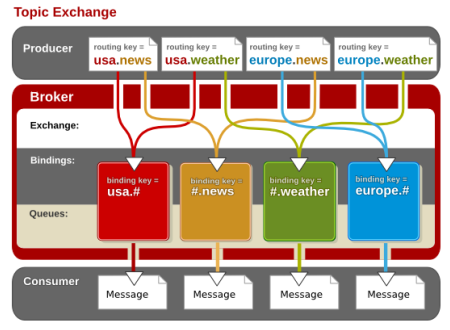
\includegraphics[scale=0.6]{\amqp}\\[0.65ex]
    \caption{Interprozesskommunikation mit Messaging-Queues}
    \label{fig:redHatCom}
\end{figure}

\textbf{Prüfungsausschuss:} Tatjana Goebel, Ali Hafezi, Ralf Merettig\\
\textbf{Abgabetermin:} \abgabeOrt{}, den \abgabeTermin\\[3ex]

\includegraphics[scale=0.45]{\betriebLogo}\\
\betriebName{}\\
\betriebAnschrift{}, \betriebOrt\\[2.5ex]
\end{center}

\small
\noindent
Dieses Werk einschließlich seiner Teile ist \textbf{urheberrechtlich geschützt}.
Jede Verwertung außerhalb der engen Grenzen des Urheberrechtsgesetzes ist ohne Zustimmung des Autors unzulässig und strafbar.
Das gilt insbesondere für Vervielfältigungen, Übersetzungen, Mikroverfilmungen sowie die Einspeicherung und Verarbeitung in elektronischen Systemen.

\end{titlepage}

\cleardoublepage

% Preface --------------------------------------------------------------------
\phantomsection
\pagenumbering{Roman}
\pdfbookmark[1]{Inhaltsverzeichnis}{inhalt}
\tableofcontents
\cleardoublepage

\phantomsection
\listoffigures
\cleardoublepage

\phantomsection
\listoftables
\cleardoublepage

\phantomsection
\lstlistoflistings
\cleardoublepage

\newcommand{\abkvz}{Abkürzungsverzeichnis}
\renewcommand{\nomname}{\abkvz}
\section*{\abkvz}
\markboth{\abkvz}{\abkvz}
\addcontentsline{toc}{section}{\abkvz}
% !TEX root = Projektdokumentation.tex

% Es werden nur die Abkürzungen aufgelistet, die mit \ac definiert und auch benutzt wurden. 
%
% \acro{VERSIS}{Versicherungsinformationssystem\acroextra{ (Bestandsführungssystem)}}
% Ergibt in der Liste: VERSIS Versicherungsinformationssystem (Bestandsführungssystem)
% Im Text aber: \ac{VERSIS} -> Versicherungsinformationssystem (VERSIS)

% Hinweis: allgemein bekannte Abkürzungen wie z.B. bzw. u.a. müssen nicht ins Abkürzungsverzeichnis aufgenommen werden
% Hinweis: allgemein bekannte IT-Begriffe wie Datenbank oder Programmiersprache müssen nicht erläutert werden,
%          aber ggfs. Fachbegriffe aus der Domäne des Prüflings (z.B. Versicherung)

% Die Option (in den eckigen Klammern) enthält das längste Label oder
% einen Platzhalter der die Breite der linken Spalte bestimmt.
\begin{acronym}[WWWWW]
	\acro{AO}{\textsc{Alte Oldenburger} Krankenversicherung AG}
	\acro{API}{Application Programming Interface}
	\acro{CSS}{Cascading Style Sheets}
	\acro{CSV}{Comma Separated Value}
	\acro{EPK}{Ereignisgesteuerte Prozesskette}
	\acro{ERM}{En\-ti\-ty-Re\-la\-tion\-ship-Mo\-dell}
	\acro{HTML}{Hypertext Markup Language}\acused{HTML}
	\acro{IDE}{Integrated Development Environment}
	\acro{MVC}[MVC]{Model View Controller}
	\acro{NatInfo}[\textsc{NatInfo}]{Natural Information System}
	\acro{Natural}[\textsc{Natural}]{Programmiersprache der Software AG}\acused{Natural}
	\acro{ORM}{Object-Relational Mapping}
	\acro{PHP}{Hypertext Preprocessor}
	\acro{SDK}{Software Development Kit}
	\acro{SQL}{Structured Query Language}
	\acro{SVN}{Subversion}
	\acro{UML}{Unified Modeling Language}
	\acro{XML}{Extensible Markup Language}
\end{acronym}

\clearpage

% Inhalt ---------------------------------------------------------------------
\pagenumbering{arabic}
% !TEX root = Projektdokumentation.tex
% !TEX root = ../Projektdokumentation.tex
\section{Einleitung}
\label{sec:Einleitung}
% TODO: Zitat finden, in dem es um den Wert der eigenständigen Projektarbeit geht, und dann hier einfügen.

\subsection{Projektumfeld} 
\label{sec:Projektumfeld}
    % Kurze Vorstellung des Ausbildungsbetriebs (Geschäftsfeld, Mitarbeiterzahl \usw)
\paragraph*{Unternehmen: } "Das OSZ IMT  in der Haarlemer Straße in Berlin-Britz im Bezirk Neukölln ist eines von 36 Oberstufenzentren in Berlin. Es vereint das Berufliche Gymnasium, die Berufsoberschule, die Fachoberschule, die Berufsfachschule, die Fachschule und die Berufsschule. (\dots)
[An ihm] arbeiten etwa 160 Lehrkräfte und nichtpädagogisches Personal in Laboren, Werkstätten, Lernbüros und allgemeinen Unterrichtsräumen. (\dots)
[Es] hat rund 3000 Schüler (\dots) [und] ist die größte Schule Berlins für Informationstechnik und Deutschlands größte Schule für Medizintechnik."\footnote{Porträt des OSZ IMT, \cite{oszimtDe} }
Wir besuchen dort seit 2 \bzw 1.5 Jahren den Unterricht der Klasse \ac{FA54}.
% Wer ist Auftraggeber/Kunde des Projekts?
\paragraph*{Auftraggeber: } Als angehende Fachinformatiker für Anwendungsentwicklung am \ac{OSZ IMT} sollen wir nun im Rahmen des Faches \ac{P/LZ} ein auf mittelständige Unternehmen anwendbares \ac{IT}-Sicherheitskonzept entwickeln. Dazu werden wir im Verlauf des Projektunterrichtes eine \ac{DMZ} unter Verwendung des zuvor in \ac{ITS} erlernten Wissens über Netzwerktechnik einrichten.  Gleichzeitig erarbeiten wir uns Anhand eines Online-Kurses der Cisco-Networking-Academy die für das Projekt benötigten Grundkenntnisse im Umgang mit Linux.\\
Verantwortlicher Auftraggeber und unser Ansprechpartner für dieses Projekt ist \textbf{Herr Ralf Henze}, Netzwerktechniker und Lehrer am \ac{OSZ IMT} in den Unterrichtsfächern \ac{ITS} und \ac{P/LZ}.

\subsection{Projektziel} 
\label{sec:Projektziel}
% Worum geht es eigentlich?
\paragraph*{Projekthintergrund: } Neben dem offensichtlichen Ziel dieses Projektes, ein \ac{DMZ}-Netzwerk unter Linux einzurichten, will es uns als Teil des Berufsschulunterrichtes natürlich vor allem etwas beibringen. So ist die eigentliche Projektarbeit durchzogen von unterschwelligem Langzeitnutzen für unsere berufliche Entwicklung. Das Wissen, wie und wo man jederzeit Befehle nachschlagen kann, die beneidenswerten Möglichkeiten mit grep, pipes und kleinen Tools wie xargs erstaunlich komplizierte Probleme lösen zu können. Auch die bewusst schon fast aufs Niveau der \ac{IHK} angehobenen Anforderungen an die Projektdokumentation und das Nahelegen, für deren Erstellung mit einer Sprache wie \LaTeX{} zu arbeiten, anstelle dies mit gängigen Office Paketen zu tun, waren eine gute Vorbereitung und hervorragende Übung. So konnte Gelerntes durch praktisches Anwenden gefestigt und Neues sinnvoll ausprobiert werden. 
% Was soll erreicht werden?
\paragraph*{Ziel des Projekts: } Die eigentliche Kernaufgabe des Projektes ist die Planung und praktische Umsetzung eines grundlegenden \ac{IT}-Sicherheitskonzeptes mit Hilfe eines \ac{DMZ}-Netzwerkes und dessen Absicherung durch das Setzen \bzw Löschen von Firewall-Regeln über ein Shell-Script. Die demilitarisierte Zone soll zwischen den Windows-Clients des Kunden im internen Netz und den potentiell schädlichen Anfragen der restlichen Welt aus dem externen Netzwerk liegen. Hier steht auch der Windows-Webserver des Kunden, welcher sowohl von Innen (zur Wartung) wie auch von Außen (für Besucher) erreichbar sein muss. Zwei virtuelle Linuxmaschinen sollen als Router zwischen den Netzen konfiguriert werden, wobei der Äußere sowohl \ac{NAT} als auch die Funktion der Firewall übernehmen soll. Planung und Umsetzung sollen umfassend Dokumentiert werden. Jedes Gruppenmitglied soll ein Kompetenzprtfolio führen, in dem er seine Kenntnisse, Gelerntes und Probleme vor, während und nach den Aufgaben der Projektarbeit sammelt und kritisch analysiert.

\subsection{Projektbegründung} 
\label{sec:Projektbegruendung}
% Warum ist das Projekt sinnvoll (\zB Kosten- oder Zeitersparnis, weniger Fehler)?
\paragraph*{Nutzen des Projekts: } Neben dem bereits mehrfach erwähnten Lerneffekt für uns als Schüler, sowohl in den Grundlagen der \ac{IT}-Sicherheit, des Arbeitens auf dem Linux-Filesystem mit Hilfe der \ac{CLI}, wie auch der Wiederholung der Befehle zur Konfiguration von Netzwerken und Schnittstellen in einer neuen leicht anderen Syntax, liegt der Projektnutzen wohl vor Allem auf dem Verstehen der Arbeitsweise von Access-Control-Listen, der Bedeutung der drei Chains sowie eines besseren Einblicks in die Welt der Linux-Distributionen, deren Stärken und Schwächen sowie deren Konfiguration. Und da das Projekt den Auftraggeber faktisch nichts kostet, uns aber fachlich weiter bringt, ist dessen Durchführung für beide Seiten ein Win-Win-Geschäft.
% Was ist die Motivation hinter dem Projekt?
\paragraph*{Motivation: } Unser Auftraggeber ist daran interessiert, ein fertiges, funktionierendes System zu erhalten, welches seine Wünsche und Anforderungen erfüllt, aber er und auch wir können uns selbst an greifbaren Indikatoren unsere bisher erworbene Fachkompetenz bewerten. Wir stellen uns somit einer solchen Aufgabe, um etwas neues zu lernen, etwas zu wiederholen und uns zu verbessern. Oder einfach, weil wir es können. Manchmal auch, um uns auf eine Zertifizierung vorzubereiten.

\subsection{Projektschnittstellen} 
\label{sec:Projektschnittstellen}
% Mit welchen anderen Systemen interagiert die Anwendung (technische Schnittstellen)?
Technisch gesehen interagieren in unserem Projekt zwei oder mehrere Windows-Rechner, welche über das Labornetzwerk des Raumes 3.1.01 verbunden sind. Auf beiden läuft jeweils eine Linux Debian Distribution in einer virtuellen Umgebung durch den VMWare Player. Die Schnittstellen der virtuellen Linuxdistributionen wiederum sind über den Bridged Modus in den Netzwerkeinstellungen des VMWare Players mit einer der physikalischen Netzwerkschnittstelle des Host-\ac{PC}s verbunden. Über das Labornetz kann Verbindung zu den Rechnern der anderen Gruppen aufgenommen werden.
% Wer genehmigt das Projekt \bzw stellt Mittel zur Verfügung? 
Die Unterrichtszeit für das Projekt, sowie die Infrastruktur (Pro Gruppe 2 Rechner + benötigte Peripherie, 2 virtuelle Maschinen und alle sonst benötigten Ressourcen, Zugang zum Internet und ins Labornetz) und alles weitere wird uns im Rahmen des \ac{P/LZ}-Unterrichtes zur Verfügung gestellt.
% Wer sind die Benutzer der Anwendung?
Dank der theoretischen Natur des Projektes sind die einzigen Benutzer unseres Projektes wir, evtl. unsere Mitschüler während des Erfahrungsaustausches untereinander, sowie unser Auftraggeber, Herr Henze, der sich immer wieder über den aktuellen Stand informiert und auch die finale Abnahme des Projektes übernimmt. 
% Wem muss das Ergebnis präsentiert werden?
Zur finalen Abnahme durch den Kunden sollen sowohl die Funktionalität der Firewall-Regeln nachweislich testbar sein, als auch die Projektdokumentation inkl. einer Kopie des verwendeten Firewall-Scriptes, den tabellarisch erfassten Testresultaten sowie je eines Kompetenzportfolios pro Gruppenmitglied zur Abgabe vorliegen.

\subsection{Projektabgrenzung} 
\label{sec:Projektabgrenzung}

\paragraph*{Was dieses Projekt nicht bietet: } Dieses Projekt will auf keinen Fall den Anspruch erheben, durch die verwendeten Techniken ein Netzwerk oder System perfekt und allumfassend vor unbefugtem Eindringen schützen zu können. Es vermittelt nur Einblicke in die Grundlagen der Netzwerktechnik und \ac{IT}-Sicherheit. Ein perfektes und vor allen schädlichen Einflüssen geschütztes System kann es nicht geben. Weiterführende Informationen zur Verbesserung der Systemsicherheit können aber der im Quellverzeichnis angegebenen Literatur entnommen werden.
% !TEX root = ../Projektdokumentation.tex
\section{Projektplanung} 
\label{sec:Projektplanung}

Da unser Projekt über die Dauer eines ganzen Schuljahres angelegt ist und wir die Unterrichtszeit zum Teil mit dem Erlernen von Fertigkeiten im Umgang mit Linux verbringen werden, muss der Ablauf genau geplant werden. Im folgenden erläutern wir die einzelnen Projektphasen, welche Ressourcen genutzt wurden und wann die Durchführung von der Planung abgewichen ist.

\subsection{Projektphasen}
\label{sec:Projektphasen}
% In welchem Zeitraum und unter welchen Rahmenbedingungen (\zB Tagesarbeitszeit) findet das Projekt statt?
Im Rahmen des \ac{P/LZ} Unterrichts erhalten wir in jeder Schulwoche meist Freitags für je zwei Blöcke a 90 Minuten Zugang zum Labor 3.1.01 am \ac{OSZ IMT} in Berlin. Das Schuljahr umfasst 14 Schulwochen in denen das Projekt durchgeführt werden muss. Außerhalb der Schulzeit können wir Private Ressourcen nutzen und planen pro Schulwoche jeweils 6 Stunden Freizeit am Wochenende als zusätzliche Pufferzeit ein. Die 42 Laborstunden und die Pufferzeit von 84 Stunden ergeben eine Gesamtzeit von 126 Stunden bis zur Projektabgabe.
% Verfeinerung der Zeitplanung, die bereits im Projektantrag vorgestellt wurde.
Wir gehen davon aus die grundlegende Planung und Analyse in den ersten beiden Schulwochen durchzuführen, die nächsten drei Schulwochen sollte das Netzwerk entworfen und erstellt werden. Anschließend wollen wir mit der Implementierung der Firewall beginnen, wofür wir \ca vier Schulwochen einplanen. Die Restliche Schulzeit wird für die Erstellung der Dokumentation und eine Stunde für die Abnahme durch den Kunden verplant. Je nach Bedarf kann die Pufferzeit zu weiterer Recherche zuhause genutzt werden.

\subsection{Zeitplanung}
\label{sec:Zeitplanung}

Tabelle~\ref{tab:Zeitplanung} zeigt unsere grobe Zeitplanung für die jeweils bevorstehenden Projektphasen:
\tabelle{Zeitplanung}{tab:Zeitplanung}{ZeitplanungKurz}

\subsection{Abweichungen vom Projektantrag}
\label{sec:AbweichungenProjektantrag}

% Sollte es Abweichungen zum Projektantrag geben (\zB Zeitplanung, Inhalt des Projekts, neue Anforderungen), müssen diese explizit aufgeführt und begründet werden.
Aufgrund unserer Unerfahrenheit im Umgang mit \LaTeX{} gestaltet sich die Erstellung der Projektdokumentation leider schwieriger als vermutet. Zudem konnten die Funktionstests an unserer Firewall nicht bis zum Ende des letzten Unterrichtsblockes abgeschlossen werden, worauf Herr Krüger viel Zeit damit verbracht hat, eine zweite Testumgebung für unser Firewall-Script mit Windows Server 2016 zu virtualisieren, deren Installation und Konfiguration im Anhang dokumentiert wurde. Deshalb erbaten wir  eine kurzzeitige Verlängerung der Abgabefrist und konnten nur die während des Unterrichtes erstellte und benutzte Dokumentation einsenden, zu finden im \Anhang {app:Anleitung}.

\subsection{Ressourcenplanung}
\label{sec:Ressourcenplanung}

% Detaillierte Planung der benötigten Ressourcen (Hard-/Software, Räumlichkeiten \usw).
% \Ggfs sind auch personelle Ressourcen einzuplanen (\zB unterstützende Mitarbeiter).
% Hinweis: Häufig werden hier Ressourcen vergessen, die als selbstverständlich angesehen werden (\zB PC, Büro).
Für die Durchführung im Labor werden benötigt: 2 Rechner mit Windows (und einem Benutzeraccount mit Adminrechten), die Software VMWare Player, eine Distribution von Debian für die virtuelle Maschine, Zugang zum Labornetz, ein Webserver und ein Editor zum Bearbeiten von \ac{HTML}, Zugang zum Internet für Recherche, Software zum Festhalten der Ergebnisse, Software zum Durchführen von Tests. Zusätzlich bedarf es der Unterstützung durch fachkundige Mitschüler wie den Herren Habekost, Schernekau und Mahnke sowie Hilfe durch Herrn Henze bei schwereren Problemen.
Für die Arbeit außerhalb der Schule haben wir zur Recherche und für weitere Versuche sowohl Rechner mit Ubuntu 14.04 als auch Rechner mit Windows 7 und 10 und eigene Heimnetzwerke mit Internetanbindung. Auch die benötigte Software sowie \LaTeX{} und Editoren um die Dokumentation anzufertigen sind vorhanden. Dank einer während des Projektes angelegten Schritt-für-Schritt Anleitung zum Einrichten des Netzwerks, sowie der Möglichkeit virtuelle Maschinen zu kopieren bzw. das Versuchsnetzwerk selbst zu virtualisieren, kann auch zuhause gearbeitet werden.

\subsection{Entwicklungsprozess}
\label{sec:Entwicklungsprozess}

% Welcher Entwicklungsprozess wird bei der Bearbeitung des Projekts verfolgt (\zB Wasserfall, agiler Prozess)?
Um unser Projekt durchzuführen benutzen wir einen auf dem Wasserfallmodel basierenden Entwicklungsprozess und den üblichen Stufen Anforderung, Entwurf, Implementation, Überprüfung und Wartung.

% !TEX root = ../Projektdokumentation.tex
\section{Analysephase} 
\label{sec:Analysephase}
% Überblick
Im Nachfolgenden verzichten wir auf einen Großteil der üblichen Berechnungen zur Wirtschaftlichkeit des Projektes, da dieses zum Großteil unserer fachlichen Kompetenzbildung dienen soll. Darüber hinaus wäre für ein fiktives mittelständisches Unternehmen ein bereits existierendes Produkt sowohl vom zu erwartenden Arbeitsaufwand wie auch finanziell deutlich günstiger. Es wird daher lediglich eine Beispielhafte Kostenberechnung für die Umsetzung der Planung durch uns erstellt und dafür ein größeres Augenmerk auf Anforderungen und Nutzen des Projekts gelegt. 

\subsection{Ist-Analyse} 
\label{sec:IstAnalyse}
% Wie ist die bisherige Situation (\zB bestehende Programme, Wünsche der Mitarbeiter)?
\paragraph*{Was ist vorhanden: } Im Labor sind für jedes Gruppenmitglied vorhanden: ein Bildschirmarbeitzplatz, Windows 7, Adminrechte, zwei physikalische Netzwerkinterfaces, Anschluß an Labornetzwerk und Internet, die Software VMWare Player, Debian Images auf einem Netzlaufwerk sowie ein Webserver.
% Was gilt es zu erstellen/verbessern?
\paragraph*{Was ist zu erstellen: } Zuerst muss nun von jeder Gruppe ein Netzplan erstellt werden. Dann gilt es, die Debian 7 (Wheezy) Linux-Images in virtuellen Maschinen auf beiden Rechnern mit Hilfe des VMWare Players aufzusetzen. Diese werden zu einem Outside- und einem Inside-Router konfiguriert und die geplanten Netzwerk- und Routingeinstellungen müssen sowohl an den virtuellen wie auch physikalischen Schnittstellen durchgeführt werden. Auf dem Rechner des Outside-Routers muss ein Webserver eingerichtet werden, wofür NAT und Port-Forwarding nötig sind. Zwischendurch wird es immer wieder der gezielten Recherche bedürfen. Um schließlich Zugriffe von außen zu regulieren, muss eine Firewall mit entsprechenden Regeln erstellt wwerden, die per Skript an- und abschaltbar ist. Die Funktionalität muss getestet werden und Projekt und Tests sind zu dokumentieren. Unser Lernfortschritt ist in einem Kompetenzportfolio niederzuschreiben. Gleichzeitig sind Laborübungen und Tests zu Linux-Kenntnissen zu absolvieren.

\subsection{Wirtschaftlichkeitsanalyse}
\label{sec:Wirtschaftlichkeitsanalyse}
Wie bereits Anfänglich erwähnt, lohnt sich das Projekt für ein fiktives mittelständisches Unternehmen nur bedingt.
\subsubsection{\gqq{Make or Buy}-Entscheidung}
\label{sec:MakeOrBuyEntscheidung}
% Gibt es vielleicht schon ein fertiges Produkt, dass alle Anforderungen des Projekts abdeckt?
Die Kosten für eine qualifizierte Kraft zur ständigen Wartung des Servers, die durch Dauerbetrieb anfallenden Stromkosten sowie die zusätzlichen Hardwarekosten bei einem zukünftigen Upscaling übersteigen bei weitem die Kosten für einen fachkundig und sicher Administrierten Server bei einem seriösen Hosting-Anbieter.
% Wenn ja, wieso wird das Projekt trotzdem umgesetzt?
\subparagraph*{} Da unsere Empfehlung an den Kunden ein Produkt eines anderen Anbieters wäre, wird das Projekt nur zu unserem Nutzen und der Erfahrung willen, die wir damit gewinnen, umgesetzt.
\subsubsection{Projektkosten}
\label{sec:Projektkosten}
% Welche Kosten fallen bei der Umsetzung des Projekts im Detail an (\zB Entwicklung, Einführung/Schulung, Wartung)?
Da es sich nur um ein fiktives Projekt handelt, verzichten wir auf eine detaillierte Berechnung mit Stromkosten innerhalb des Labors, den Gehältern der Lehrkräfte oder etwaiger Lizenzgebühren. Wir beschränken uns auf eine fiktive Beispielrechnung mit unserem Stundenlohn während der Projektdauer.
\paragraph*{Beispielrechnung (verkürzt): } Die realen Kosten für die Durchführung des Projekts setzen sich sowohl aus Personal-, als auch aus Ressourcenkosten zusammen. Wir rechnen hier lediglich mit dem fiktiven Gehalt eines Auszubildendem im zweiten Lehrjahr von ca. \eur{800} Brutto pro Monat. 
% Stundenlohn (brutto) = 3 × dein Monatslohn (brutto) ÷ 13 ÷ die Anzahl deiner wöchentlichen Arbeitsstunden
\begin{eqnarray}
3\cdot \eur{800}\mbox{/Monat} \div {13} \div 40 \mbox{ h/Monat} \approx \eur{4,62}\mbox{/h}
\end{eqnarray}
Es ergibt sich also ein Stundenlohn von \eur{4,62}. Die Durchführungszeit des Projekts beträgt 42 Stunden. Die Nutzung von Ressourcen\footnote{Räumlichkeiten, Arbeitsplatzrechner etc.} sowie die Kosten durch andere Mitarbeiter werden hier nicht mit eingerechnet. Eine Aufstellung der Kosten befindet sich in Tabelle~\ref{tab:Kostenaufstellung} und sie betragen insgesamt \eur{388,08} für zwei Entwickler bei 42 h/Monat Arbeitszeit und je einem Gehalt von \eur{800} monatlich.

\tabelle{Kostenaufstellung für 2 Entwickler/Monat}{tab:Kostenaufstellung}{Kostenaufstellung.tex}

\subsubsection{Amortisationsdauer}
\label{sec:Amortisationsdauer}
% Welche monetären Vorteile bietet das Projekt (\zB Einsparung von Lizenzkosten, Arbeitszeitersparnis, bessere Usability, Korrektheit)?
% Wann hat sich das Projekt amortisiert?
Aufgrund unserer \gqq{Make or Buy}-Entscheidung und da das Projekt nur zu Lernzwecken umgesetzt wird verzichten wir hier auf die Berechnung eines fiktiven Rentabilitätszeitpunktes. Das gelernte wird sich spätestens zur IHK-Prüfung und bei der Anfertigung der Dokumentation des IHK-Abschlussprojektes auszahlen.

\subsection{Nutzwertanalyse}
\label{sec:Nutzwertanalyse}
% Darstellung des nicht-monetären Nutzens (\zB Vorher-/Nachher-Vergleich anhand eines Wirtschaftlichkeitskoeffizienten). 
Durch den Aufbau einer DMZ können wir die Zugriffe auf unsere Server, in diesem Fall ein einfacher Webserver, von Außen und Innen reglementieren. So wird über den Routern mit einer konfigurierten Firewall ein sicherer Zugang zu unserem Webserver ermöglicht. Die Aufteilung in unterschiedliche Netzwerke ermöglicht den Administratoren eine einfachere Verwaltung der Berechtigungen für die Mitglieder des Firmennetzes.

%\paragraph{Beispiel}
%Ein Beispiel für eine Entscheidungsmatrix findet sich in Kapitel~\ref{sec:Architekturdesign}: \nameref{sec:Architekturdesign}.

\subsection{Qualitätsanforderungen}
\label{sec:Qualitaetsanforderungen}
% Welche Qualitätsanforderungen werden an die Anwendung gestellt (\zB hinsichtlich Performance, Usability, Effizienz \etc (siehe \citet{ISO9126}))?
Der Webserver soll von Außen (über die öffentliche IP-Adresse des Outside-Routers) und Innen erreichbar, aber vor unbefugten Zugriffen potentieller Angreifer mit den uns zur Verfügung stehenden Mitteln geschützt werden. Es muss also sichergestellt werden, dass kein unberechtigter Dritter administrativen Zugriff auf die Geräte und deren Konfiguration hat. Dabei ist darauf zu achten, dass die Mitarbeiter mit entsprechender Berechtigung (also zum Beispiel von einem Admin-PC aus dem inneren Netz aus) weiterhin Zugriff auf das Internet und den Webserver in der DMZ haben.

\subsection{Lastenheft}
\label{sec:Lastenheft}
% Auszüge aus dem Lastenheft/Fachkonzept, wenn es im Rahmen des Projekts erstellt wurde.
% Mögliche Inhalte: Funktionen des Programms (Muss/Soll/Wunsch), User Stories, Benutzerrollen

\paragraph*{Die Mitarbeiter} sollen untereinander, mit dem Webserver und dem Internet kommunizieren können, dabei jedoch bestmöglich geschützt werden.
\paragraph*{Die Administrator} sollen zusätzlich die Möglichkeit haben, die Server und Router aus der Ferne zu warten. Dabei sollte es unerheblich sein, wie viele Clients und Server sich im internen \bzw DMZ-Netz befinden.

%\paragraph{Beispiel}
Einen genaueren Überblick über die festgestellten Anforderungen an die einzelnen Teile der DMZ findet sich in unserem ausführlichen Lastenheft im \Anhang{app:Lastenheft}. 

\Zwischenstand{Analysephase}{Analyse}

% !TEX root = ../Projektdokumentation.tex
\section{Entwurfsphase} 
\label{sec:Entwurfsphase}

% Erklärung
Da unsere Hard- und Software von unserem Auftraggeber gestellt und vorgegeben wird, erübrigt seine ausführliche Begründung, weshalb wir diese Materialien verwendet haben. Zudem wird so sichergestellt, dass während unserer Projektzeit alle benötigten Mittel zur Verfügung stehen.

\subsection{Zielplattform}
\label{sec:Zielplattform}

\paragraph*{Hardware: } 
Die uns zur Verfügung stehenden Desktop PCs bleiben unverändert. Die Leistungsdaten derer  genügen für den Aufbau einer einfachen DMZ.

\paragraph*{Software: } 
Für die Implementation eines Routers als virtuelle Maschine nutzen wir den vorinstallierten VMWare Player. Dieser ist kostenlos und berechtigt uns zum Virtualisieren einer Linux Distribution. Des Weiteren werden wir auch das beigefügte Debian benutzen. Auf den VMs wird mit BASH und Linux-Befehlen gearbeitet, da wir nur kleinere Konfigurationen und Scripts schreiben. Um die Konfiguration zu testen, die Router per Remote zu konfigurieren und eventuell Dateien auszutauschen, wird noch SSH- und FTP-Client-Software benötigt. Dafür werden wir Putty und winscp verwenden. Diese Tools sind kompakt und beeinträchtigen nicht die Leistung der Hosts.

\subsection{Netzwerkplan}
\label{sec:Geschaeftslogik}

\Abbildung{Netzplan} zeigt die grundsätzliche IP-Adressverteilung in den geplanten Netzwerken. 
Unser Konzept teilt sich grundsätzlich in das Labornetz (hier symbolisch für den Rest der Welt), das interne Netz (mit den Windows-Clients unseres Kunden) und das von der Außenwelt abgeschottete \ac{DMZ}-Netzwerk, welches nur über spezielle Berechtigungen zu erreichen und für spezielle Dienste (Webserver) zu verwenden ist.
\begin{figure}[htb]
\centering
\includegraphicsKeepAspectRatio{PLZNetzplanProjektumgebung.png}{0.9}
\caption{Netzplan DMZ Arbeitsgruppe 9}
\label{fig:Netzplan}
\end{figure}


\subsection{Maßnahmen zur Qualitätssicherung}
\label{sec:Qualitaetssicherung}
%begin{itemize}
	%\item Welche Maßnahmen werden ergriffen, um die Qualität des Projektergebnisses (siehe Kapitel~\ref{sec:Qualitaetsanforderungen}: \nameref{sec:Qualitaetsanforderungen}) zu sichern (\zB automatische Tests, Anwendertests)?
%	\item \Ggfs Definition von Testfällen und deren Durchführung (durch Programme/Benutzer).
%\end{itemize}
Bei jeder Veränderungen der Konfiguration werden Tests durchgeführt. Diese sollen gewährleisten, dass das \nameref{sec:Lastenheft} eingehalten wird. Vorgenommene Konfigurationen werden notiert und das Firewall-Script wird zusätzlich auf einen externen Datenträger kopiert. So wird sichergestellt, dass bei einem Defekt die ursprüngliche Konfiguration schnell wieder verfügbar ist.

\subsection{Pflichtenheft/Datenverarbeitungskonzept}
\label{sec:Pflichtenheft}
	%\item Auszüge aus dem Pflichtenheft/Datenverarbeitungskonzept, wenn es im Rahmen des Projekts erstellt wurde.
\begin{enumerate}

	\item Musskriterien
	
	\begin{itemize}
		\item Das DMZ-Netz erhält die Netzmaske 172.16.9.0/24
		\item Das intere Netz erhält die Netzmaske 10.0.9.0/24
		\item Die öffentliche Schnittstelle des Outside-Router erhält die IP 192.168.200.109
		\item Der Outside-Router erhält als Standard-Gateway die IP 192.168.200.1
		\item Der Outside-Router erhält eine statische Route für das interne und DMZ-Netz
		\item Der Inside-Router erhält als Standard-Gateway das Interface des Outside-Routers, welches in die DMZ zeigt
		\item Der Webserver ist über die öffentliche IP des Outside-Routers über HTTP/S von außen erreichbar
		\item Der Webserver ist über die lokale IP 172.16.9.3 über HTTP/S aus dem internen Netzwerk erreichbar
		\item Die Router und Windows-Clients bekommen als DNS-Server die IPs 192.168.95.40 und 192.168.95.41
		\item Die Router und Windows-Clients bekommen als NTP-Server die IP 192.168.200.1
		\item Die Firewall verhindert unrechtmäßigen Datentransfer zwischen den Netzen und auf den Routern
		\item Der Admin-PC mit der IP 10.0.9.2 ist berechtigt mittels SSH auf die Router zuzugreifen	
	\end{itemize}
	
	\item Kannkriterien
	
	\begin{itemize}
		\item Die Firewall lässt sich mit den Optionen "start" und "stop" an- bzw.\ ausschalten
		\item Die Firewall-Scripts der Router befinden sich im Verzeichnis /root/bin
		\item Die Veränderung der Firewall-Konfiguration befindet sich jeweils im Verzeichnis /var/log/firewall
		\item Der Admin-PC mit der IP 10.0.9.2 ist berechtigt mittels RDP auf den Webserver zuzugreifen
	\end{itemize}
\end{enumerate}

%\paragraph{Beispiel}
%Ein Beispiel für das auf dem Lastenheft (siehe Kapitel~\ref{sec:Lastenheft}: \nameref{sec:Lastenheft}) aufbauende Pflichtenheft ist im \Anhang{app:Pflichtenheft} zu finden.


\Zwischenstand{Entwurfsphase}{Entwurf}

% !TEX root = ../Projektdokumentation.tex
\section{Implementierungsphase} 
\label{sec:Implementierungsphase}
Bevor mit der eigentlichen Programmierung und Implementierung begonnen werden kann, muss direkt am Anfang eine dazugehörige Entwicklungsumgebung aufgesetzt werden. Dies war zum Zeitpunkt des Projektantrags nicht bekannt. 
Während der gesamten Dauer das Projekts wurde regelmäßig über die Versionsverwaltungssoftware Github gesichert.

\subsection{Implementierung der Projektumgebung}
\label{subsec:ImplementierungDatenstruktur}
% Beschreibung der angelegten Datenbank (z.B. Generierung von SQL aus Modellierungswerkzeug oder händisches Anlegen), XML-Schemas usw..
Nach einem Backup des bisherigen Systems auf einem MacBook Pro, werden Ruby, Rails und alle weiteren benötigten Frameworks und Bibliotheken mit den bekannten Informationen eingebunden und deren Funktionstüchtigkeit getestet. Der MySQL-Server, Ruby Version Manager (rvm), über den Ruby installiert wird, sowie das Datenbank-Management System Sequel Pro werden mit Hilfe des OS X Paket Managers Homebrew installiert. Über den Bash rails new app wird ein neues Projekt erstellt. Als Entwicklungsumbegung (IDE) wird Rubymine verwendet.


\subsection{Implementierung des Webservers und des Routings}
\label{subsec:ImplementierungBenutzeroberfläche}
% Beschreibung der Implementierung der Benutzeroberfläche, falls dies separat zur Implementierung der Geschäftslogik erfolgt (z.B. bei HTML-Oberflächen und Stylesheets).
% Ggfs. Beschreibung des Corporate Designs und dessen Umsetzung in der Anwendung.
% Screenshots der Anwendung
Als Web Server wird Thin verwendet, welcher leicht als RubyGem über Ruby installiert werden kann und keiner weiteren Konfiguration bedarf. In der Projektdatei config/routes.rb werden die Routen zum Controller mit den entsprechenden Operationen definiert.

\subsection{Implementierung der Datenbank}
\label{subsec:ImplementierungGeschäftslogik}
% Beschreibung des Vorgehens bei der Umsetzung/Programmierung der entworfenen Anwendung. 
% Ggfs. interessante Funktionen/Algorithmen im Detail vorstellen, verwendete Entwurfsmuster zeigen. 
% Quelltextbeispiele zeigen. 
% Hinweis: Wie in Kapitel 1: Einleitung zitiert, wird nicht ein lauffähiges Programm bewertet, sondern die Projektdurchführung. Dennoch würde ich immer Quelltextausschnitte zeigen, da sonst Zweifel an der tatsächlichen Leistung des Prüflings aufkommen können.
% Beispiel Die Klasse ComparedNaturalModuleInformation findet sich im Anhang A.11: Klasse: ComparedNaturalModuleInformation auf Seite xv.
Nach der Erstellung eines Projekts wird über den simplen Befehl rake db:create 
die Datenbank erstellt werden und danach das vom externen Entwickler erhaltene MySQL-Skript importiert. Migrationen für die neuen Tabellen werden in Rails geschrieben und über rake db:migrate der Datenbank hinzugefügt. Das hat den Vorteil, dass man jederzeit seine selbst erstellten Migrationen zurücksetzen, diese editieren und der Datenbank wieder hinzufügen kann. Über ein erstelltes MySQL-Skript werden dann die Daten für die Tabellen der Dropdown Menüs importiert.

\subsection{Implementierung der Models}
Für jede Tabelle der Datenbank wird eine Klasse erstellt. Dies geschieht über den Befehl rails generate model [Tabellenname]. Dabei ist darauf zu achten, dass man sich an den Namenskonventionen von Rails orientiert. Rails kann so die entsprechenden Modelle der jeweiligen Tabelle automatisch zuordnen und die Datenbankabfragen generieren. Danach werden in den Model-Klassen die Relationen der Klassen nach dem Vorbild der Tabellen untereinander definiert und Operationen zur Gültigkeitsprüfung der an die Tabelle zu übergebenen Daten geschrieben.

\subsection{Implementierung des Fachkonzepts}
Über den Befehl rails generate controller [Controllername] wird eine neue Klasse für die entsprechenden Controller erstellt. Entsprechend der Namenskonventionen werden durch Rails zusätzliche Hilfsdateien, sowie einen Pfad zur View des Controllers angelegt. Anhand der Methodennamen erfolgt das Routing zu dessen Operationen. Des Weiteren wird anhand der Rails-Namenskonvention auch die entsprechende Ansicht festgelegt. Hier werden die entsprechenden CRUD – Operationen implementiert. 

\subsection{Implementierung der Benutzeroberfläche}
Für die Ansicht der Projekte und Teilprojekte werden nur die nötigsten Dateien und Links für die Weiterleitung zum Materialeingangsbericht implementiert. Die Ansichten für den Bericht werden mit der HTML – Abstraktionssprache HAML geschrieben. Über die Index-Datei des Berichts werden alle zu dem Teilprojekt aufgelisteten gespeicherten Berichte angezeigt und zu den entsprechenden Ansichten (Anzeigen, Bearbeiten, Löschen) verlinkt. Zudem wird ein Link zur Erstellung eines neuen Berichts generiert. Für das Anzeigen, Bearbeiten und Erstellen wird jeweils das gleiche „Partial“ – Formular mit einem Parameter für das Aktivieren bzw. Deaktivieren geladen. Die Datenauswahl in den Dropdown-Menüs werden über Rails geladen.

\Zwischenstand{Implementierungsphase}{Implementierung}

% !TEX root = ../Projektdokumentation.tex
\section{Abnahmephase} 
\label{sec:Abnahmephase}
Da die Originalmaschinen zum Testzeit nicht mehr verfügbar waren, wurde hierzu eine eigene Testumgebung mittels HyperV nachgestellt. Genauere Angaben über die Teststellung und ein ausführlicher Test befinden sich im Anhang B.

\subparagraph*{} Der Zugang zum Webserver ohne aktivierter Firewall konnte bereits abgenommen werden.

\Zwischenstand{Abnahmephase}{Abnahme}

% !TEX root = ../Projektdokumentation.tex
\section{Einführungsphase}
\label{sec:Einfuehrungsphase}
\subsection{Geplante Einführung}
\label{subsec:EinführungGeplant}
Die tatsächliche Inbetriebnahme der Anwendung kann derzeit noch nicht erfolgen, da dieses Projekt abhängig von der Integration in Copper ist.

\subsection{Benutzerschulung} Einführung bei den Mitarbeitern
Den Sounddesignern wird das Projekt demonstriert und die Bedienung erklärt.

\Zwischenstand{Einführungsphase}{Einfuehrung}

% !TEX root = ../Projektdokumentation.tex
\section{Dokumentation}
\label{sec:Dokumentation}
% Wie wurde die Anwendung für die Benutzer/Administratoren/Entwickler dokumentiert (\zB Benutzerhandbuch, API-Dokumentation)?
Da unser Auftraggeber bereits früh im Projekt seine Vorliebe nach einer, den \ac{IHK}-Richtlinien entsprechend umgesetzten Dokumentation Ausdruck verlieh, beschlossen wir uns, seinem Wunsch zu entsprechen. So wurde die finale Dokumentation in \LaTeX{ } erstellt. Das Ergebnis mag sich zwar sehen lassen, dennoch schlägt die Bearbeitung der Dokumentation dank der aufgetretenen Schwierigkeiten im Umgang mit \LaTeX{} mit einem zu hohen Anteil des Zeitbudgets zu Buche. Nichtsdestotrotz hier das beschriebene Resultat. Wir hoffen, es war die Mühen wert. Zu Ihrer Erstellung wurden zusätzlich folgende Webseiten zu Hilfe gezogen: \cite{texstudio}, \cite{texbibtut} und vor allem \cite{manualdetailed}
% Hinweis: Je nach Zielgruppe gelten bestimmte Anforderungen für die Dokumentation (\zB keine IT-Fachbegriffe in einer Anwenderdokumentation verwenden, aber auf jeden Fall in einer Dokumentation für den IT-Bereich).

\paragraph*{Entwicklerdokumentation:}
Die der neben der Konfiguration angelegte Entwicklerdokumentation befindet sich im \Anhang{app:Anleitung}. Sie wurde als Schritt-für-Schritt-Anleitung zum Wiederherstellen des bereits erreichten Zustandes im Fall eines technischen Versagens geführt. Sie wurde basierend auf Informationen aus folgenden Webseiten erstellt: \cite{debianOrg12}, \cite{debianOrg5}, \cite{iptableshowto}, \cite{iptablestutorial} und \cite{nathowto} 
%Die Entwicklerdokumentation wurde mittels PHPDoc\footnote{Vgl. \cite{phpDoc}} automatisch generiert. Ein beispielhafter Auszug aus der Dokumentation einer Klasse findet sich im \Anhang{app:Doc}. 

\Zwischenstand{Dokumentation}{Dokumentation}

% !TEX root = ../Projektdokumentation.tex
\section{Fazit} 
\label{sec:Fazit}

\dots

\subsection{Soll-/Ist-Vergleich}
\label{sec:SollIstVergleich}
% Wurde das Projektziel erreicht und wenn nein, warum nicht?

\dots
%ja, viel über Netzwerk, Firewall(iptables), Linux(grundsätzliche Struktur, Terminal)
%aber nicht in der Zeit
%ne


% Ist der Auftraggeber mit dem Projektergebnis zufrieden und wenn nein, warum nicht?
% Wurde die Projektplanung (Zeit, Kosten, Personal, Sachmittel) eingehalten oder haben sich Abweichungen ergeben und wenn ja, warum?

\dots
% zeit, somit kosten
% auch aufgrund von Krankheit, begrenztem Zugang
% testabweichung

% Hinweis: Die Projektplanung muss nicht strikt eingehalten werden. Vielmehr sind Abweichungen sogar als normal anzusehen. Sie müssen nur vernünftig begründet werden (\zB durch Änderungen an den Anforderungen, unter-/überschätzter Aufwand).

%\paragraph{Beispiel (verkürzt)}
Wie in Tabelle~\ref{tab:Vergleich} zu erkennen ist, konnte die Zeitplanung bis auf wenige Ausnahmen, einige davon jedoch aus bereits unter \ref{sec:Dokumentation} erwähnten Gründen mit gravierend abweichenden Zeiten, eingehalten werden (falls der Auftraggeber bei unserer verspäteten Abgabe nochmal beide Augen zudrückt).

\tabelle{Soll-/Ist-Vergleich}{tab:Vergleich}{Zeitnachher.tex}


\subsection{Lessons Learned}
\label{sec:LessonsLearned}
% Was hat der Prüfling bei der Durchführung des Projekts gelernt (\zB Zeitplanung, Vorteile der eingesetzten Frameworks, Änderungen der Anforderungen)?

\dots
% Zeitplanung, Linux, Firewall, zusätzlich (Netzwerk-)Virtualisierung

\subsection{Ausblick}
\label{sec:Ausblick}
%  Wie wird sich das Projekt in Zukunft weiterentwickeln (\zB geplante Erweiterungen)?

\dots
%Netzwerk ausbauen, domain controller, DHCP, DNS, FTP, Exchange (über Windows und / oder Linux)


% Literatur ------------------------------------------------------------------
\clearpage
\renewcommand{\refname}{Literaturverzeichnis}
\bibliography{Bibliographie}
\bibliographystyle{Allgemein/natdin} % DIN-Stil des Literaturverzeichnisses
% !TEX root = Projektdokumentation.tex
\clearpage
\addsec{Eidesstattliche Erklärung}

% Hinweis: die eidesstattliche Erklärung ist ggfs. an die Richtlinie der IHK anzupassen

Wir, \autorNameTwo{} und \autorNameOne{}, versichern hiermit, dass wir unsere \textbf{\betreff} mit dem
Thema
\begin{quote}
\textit{\kompletterTitel}
\end{quote}
selbständig verfasst und keine anderen als die angegebenen Quellen und Hilfsmittel benutzt haben,
wobei wir alle wörtlichen und sinngemäßen Zitate als solche gekennzeichnet haben. Die Arbeit
wurde bisher keinem anderen Lehrer vorgelegt und auch nicht veröffentlicht.\\[6ex]

\abgabeOrt, den \abgabeTermin


\rule[-0.2cm]{5.5cm}{0.5pt}

\textsc{\autorNameOne, \autorNameTwo}


% Anhang ---------------------------------------------------------------------
\clearpage
\appendix
\pagenumbering{roman}
% !TEX root = Projektdokumentation.tex
% \section{Anhang}
% \subsection{Schritt-für-Schritt Anleitung}
% \label{app:Anleitung}
% gesetzt in der pagecommand-Option von \includepdf, damit die erste PDF-Seite die richtigen Header bekommt
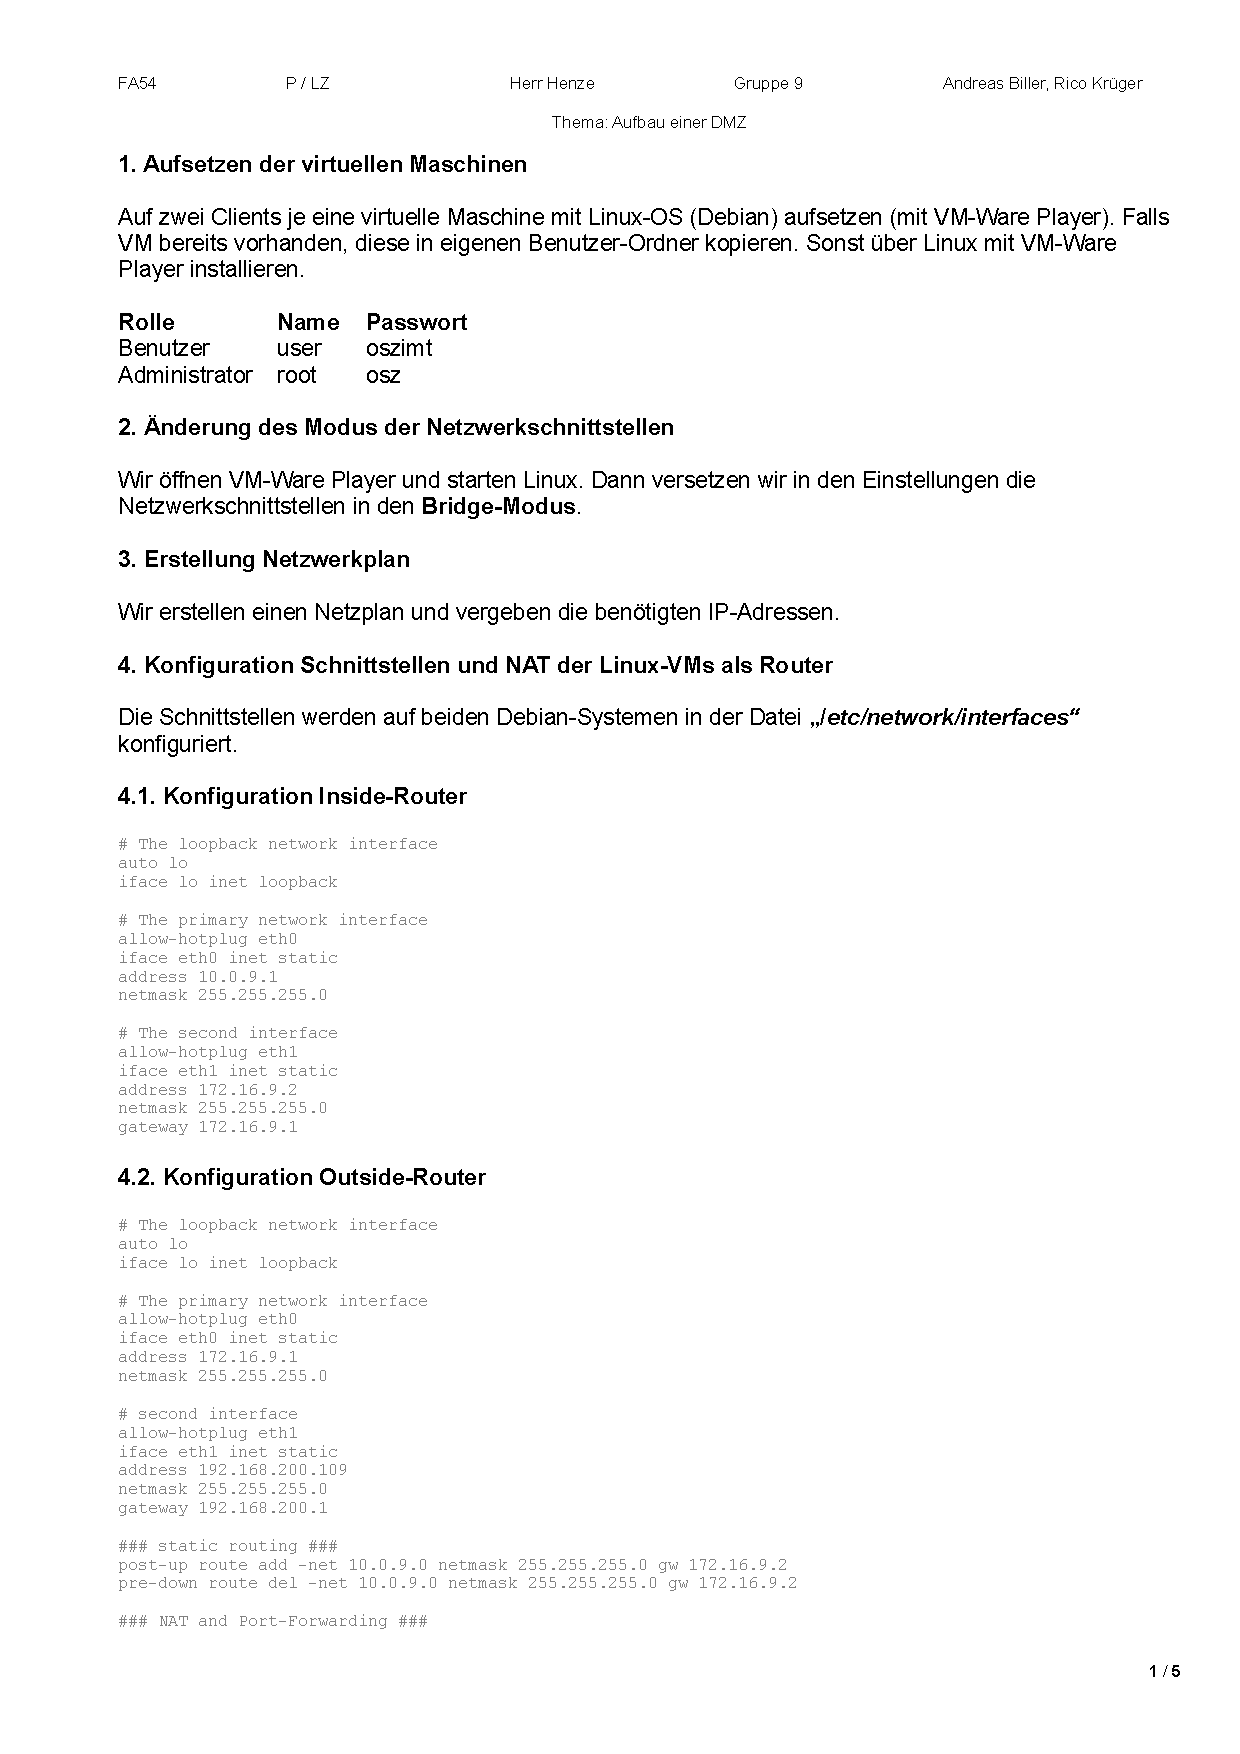
\includepdf[scale=0.8,clip,trim=0cm 0cm 0cm 0cm,offset=0 -2cm,pages={1},pagecommand={\section{Anhang}\subsection{Schritt-für-Schritt Anleitung}\label{app:Anleitung}}]{AufbauEinerDMZ.pdf}
\includepdf[scale=0.85,clip,trim=0cm 0cm 0cm 0cm,offset=0 -0.5cm,pages={2-5},pagecommand={}]{AufbauEinerDMZ.pdf}
\clearpage

\subsection{Detaillierte Zeitplanung}
\label{app:Zeitplanung}
\tabelleAnhang{ZeitplanungKomplett}
\clearpage

\subsection{Lastenheft (Auszug)}
\label{app:Lastenheft}
Es folgt ein Auszug aus dem Lastenheft mit Fokus auf die Anforderungen:

Die Anwendung muss folgende Anforderungen erfüllen: 
\begin{enumerate}[itemsep=0em,partopsep=0em,parsep=0em,topsep=0em]
\item Verarbeitung der Moduldaten
	\begin{enumerate}
	\item Die Anwendung muss die von Subversion und einem externen Programm bereitgestellten Informationen (z.B. Source-Benutzer, -Datum, Hash) verarbeiten.
	\item Auslesen der Beschreibung und der Stichwörter aus dem Sourcecode.
	\end{enumerate}
\item Darstellung der Daten
	\begin{enumerate}
	\item Die Anwendung muss eine Liste aller Module erzeugen inkl. Source-Benutzer und -Datum, letztem Commit-Benutzer und -Datum für alle drei Umgebungen. 
	\item Verknüpfen der Module mit externen Tools wie z.B. Wiki-Einträgen zu den Modulen oder dem Sourcecode in Subversion.
	\item Die Sourcen der Umgebungen müssen verglichen und eine schnelle Übersicht zur Einhaltung des allgemeinen Entwicklungsprozesses gegeben werden. 
	\item Dieser Vergleich muss auf die von einem bestimmten Benutzer bearbeiteten Module eingeschränkt werden können. 
	\item Die Anwendung muss in dieser Liste auch Module anzeigen, die nach einer Bearbeitung durch den gesuchten Benutzer durch jemand anderen bearbeitet wurden. 
	\item Abweichungen sollen kenntlich gemacht werden. 
	\item Anzeigen einer Übersichtsseite für ein Modul mit allen relevanten Informationen zu diesem.
	\end{enumerate}
\item Sonstige Anforderungen
	\begin{enumerate}
	\item Die Anwendung muss ohne das Installieren einer zusätzlichen Software über einen Webbrowser im Intranet erreichbar sein.
	\item Die Daten der Anwendung müssen jede Nacht \bzw nach jedem \acs{SVN}-Commit automatisch aktualisiert werden. 
	\item Es muss ermittelt werden, ob Änderungen auf der Produktionsumgebung vorgenommen wurden, die nicht von einer anderen Umgebung kopiert wurden. Diese Modulliste soll als Mahnung per E-Mail an alle Entwickler geschickt werden (Peer Pressure).
	\item Die Anwendung soll jederzeit erreichbar sein.
	\item Da sich die Entwickler auf die Anwendung verlassen, muss diese korrekte Daten liefern und darf keinen Interpretationsspielraum lassen.
	\item Die Anwendung muss so flexibel sein, dass sie bei Änderungen im Entwicklungsprozess einfach angepasst werden kann.
	\end{enumerate}
\end{enumerate}


\subsection{Pflichtenheft (Auszug)}
\label{app:Pflichtenheft}

\subsubsection*{Zielbestimmung}

\begin{enumerate}[itemsep=0em,partopsep=0em,parsep=0em,topsep=0em]
\item Musskriterien % Wikipedia: für das Produkt unabdingbare Leistungen, die in jedem Fall erfüllt werden müssen
	\begin{enumerate}
	\item Modul-Liste: Zeigt eine filterbare Liste der Module mit den dazugehörigen Kerninformationen sowie Symbolen zur Einhaltung des Entwicklungsprozesses an
		\begin{itemize}
		\item In der Liste wird der Name, die Bibliothek und Daten zum Source und Kompilat eines Moduls angezeigt.
		\item Ebenfalls wird der Status des Moduls hinsichtlich Source und Kompilat angezeigt. Dazu gibt es unterschiedliche Status-Zeichen, welche symbolisieren in wie weit der Entwicklungsprozess eingehalten wurde \bzw welche Schritte als nächstes getan werden müssen. So gibt es \zB Zeichen für das Einhalten oder Verletzen des Prozesses oder den Hinweis auf den nächsten zu tätigenden Schritt. 
		\item Weiterhin werden die Benutzer und Zeitpunkte der aktuellen Version der Sourcen und Kompilate angezeigt. Dazu kann vorher ausgewählt werden, von welcher Umgebung diese Daten gelesen werden sollen. 
		\item Es kann eine Filterung nach allen angezeigten Daten vorgenommen werden. Die Daten zu den Sourcen sind historisiert. Durch die Filterung ist es möglich, auch Module zu finden, die in der Zwischenzeit schon von einem anderen Benutzer editiert wurden.
		\end{itemize}
	\item Tag-Liste: Bietet die Möglichkeit die Module anhand von Tags zu filtern. 
		\begin{itemize}
		\item Es sollen die Tags angezeigt werden, nach denen bereits gefiltert wird und die, die noch der Filterung hinzugefügt werden könnten, ohne dass die Ergebnisliste leer wird.
		\item Zusätzlich sollen die Module angezeigt werden, die den Filterkriterien entsprechen. Sollten die Filterkriterien leer sein, werden nur die Module angezeigt, welche mit einem Tag versehen sind.
		\end{itemize}
	\item Import der Moduldaten aus einer bereitgestellten \acs{CSV}-Datei
		\begin{itemize}
		\item Es wird täglich eine Datei mit den Daten der aktuellen Module erstellt. Diese Datei wird (durch einen Cronjob) automatisch nachts importiert.
		\item Dabei wird für jedes importierte Modul ein Zeitstempel aktualisiert, damit festgestellt werden kann, wenn ein Modul gelöscht wurde.
		\item Die Datei enthält die Namen der Umgebung, der Bibliothek und des Moduls, den Programmtyp, den Benutzer und Zeitpunkt des Sourcecodes sowie des Kompilats und den Hash des Sourcecodes.
		\item Sollte sich ein Modul verändert haben, werden die entsprechenden Daten in der Datenbank aktualisiert. Die Veränderungen am Source werden dabei aber nicht ersetzt, sondern historisiert.
		\end{itemize}
	\item Import der Informationen aus \ac{SVN}. Durch einen \gqq{post-commit-hook} wird nach jedem Einchecken eines Moduls ein \acs{PHP}-Script auf der Konsole aufgerufen, welches die Informationen, die vom \ac{SVN}-Kommandozeilentool geliefert werden, an \acs{NatInfo} übergibt.
	\item Parsen der Sourcen
		\begin{itemize}
		\item Die Sourcen der Entwicklungsumgebung werden nach Tags, Links zu Artikeln im Wiki und Programmbeschreibungen durchsucht.
		\item Diese Daten werden dann entsprechend angelegt, aktualisiert oder nicht mehr gesetzte Tags/Wikiartikel entfernt.
		\end{itemize}
	\item Sonstiges
		\begin{itemize}
		\item Das Programm läuft als Webanwendung im Intranet.
		\item Die Anwendung soll möglichst leicht erweiterbar sein und auch von anderen Entwicklungsprozessen ausgehen können.
		\item Eine Konfiguration soll möglichst in zentralen Konfigurationsdateien erfolgen.
		\end{itemize}
	\end{enumerate}
\end{enumerate}

\subsubsection*{Produkteinsatz}

\begin{enumerate}[itemsep=0em,partopsep=0em,parsep=0em,topsep=0em]
\item{Anwendungsbereiche\\
Die Webanwendung dient als Anlaufstelle für die Entwicklung. Dort sind alle Informationen für die Module an einer Stelle gesammelt. Vorher getrennte Anwendungen werden ersetzt \bzw verlinkt.}
\item{Zielgruppen\\
\NI wird lediglich von den \ac{Natural}-Entwicklern in der EDV-Abteilung genutzt.}
\item{Betriebsbedingungen\\ % Wikipedia: physikalische Umgebung des Systems, tägliche Betriebszeit, ständige Beobachtung des Systems durch Bediener oder unbeaufsichtigter Betrieb
Die nötigen Betriebsbedingungen, also der Webserver, die Datenbank, die Versionsverwaltung, das Wiki und der nächtliche Export sind bereits vorhanden und konfiguriert. Durch einen täglichen Cronjob werden entsprechende Daten aktualisiert, die Webanwendung ist jederzeit aus dem Intranet heraus erreichbar.}
\end{enumerate}

\clearpage

\subsection{Netzpläne}
\label{app:Netzplan}
Der Netzplan unserer DMZ in der Projektumgebung:
\begin{figure}[htb]
\centering
\includegraphicsKeepAspectRatio{PLZNetzplanProjektumgebung.png}{0.8}
\caption{Netzplan der DMZ (Arbeitsgruppe 9)}
\end{figure}

Der Netzplan unserer DMZ in der Testumgebung:
\begin{figure}[htb]
    \centering
    \includegraphicsKeepAspectRatio{PLZNetzplanTestumgebung.png}{0.8}
    \caption{Netzplan der erweiterten DMZ in unserer Testumgebung}
\end{figure}
\clearpage

\section{Testdokumentation}
\label{app:Test}
\begin{table}
    \tabelleAnhang{Systeminformation}{tab:Systeminformation}{Systeminformation.tex}
    \caption{Hardwaredetails des Testsystems}
    \label{tab:tabletestsystem}
\end{table}

\subsection{Aufbau der Testumgebung}
\label{app:testaufbau}
Die zur Umsetzung dieses Kapitels benötigten Informationen entstammen unter anderem den hilfreichen Artikeln folgender Webseiten: \cite{networkdriverhacking}

\subsubsection{Implementierung der Virtuellen Maschinen}
Im Server-Manager fügen wir über \textit{Verwalten > Rollen und Features hinzufügen} den Hyper-V-Manager hinzu indem wir dem Assistenten folgen. Dieser gestattet es virtuelle Maschinen und Netzwerke zu installieren.
Als nächstes wird eine neue virtuelle Linux (Debian 7.1)  Maschine (Generation 1) aus einem Image erstellt. Dies geschieht mit Hilfe eines Assistenten. Sie bekommt einen virtuellen Prozessor und 1 \ac{GB} Arbeitsspeicher. Des weiteren wird bei der Installation eine 5 \ac{GB} große Festplatte für die Maschine erstellt und ihr zugewiesen. Als virtuellen Switch weisen wir ihr vorläufig den Netzwerkadapter des Hosts zu. Somit besitzt unsere Linux-\ac{VM} Internet. Um sie zu installieren, startet man nun die Maschine und verbindet sich zu ihr. Danach folgt man wie gewohnt den Installationsschritten wie bei einer physischen Maschine. Danach installieren wir den \ac{NTP}-Service. Ist die Grundkonfiguration fertig, wird die Maschine ausgeschaltet.
Die Installation der Windows 7 \ac{VM} erfolgt analog zu die der Linux \ac{VM}. Wir vergeben jedoch 4 \ac{GB} \ac{RAM} und erstellen eine mindestens 30 \ac{GB} große virtuelle Festplatte. Nach der Installation wird die Firewall wie in \nameref{sec:Implementierungsphase} eingerichtet. Zusätzlich werden noch nützliche Software wie putty oder winscp heruntergeladen.
Nach der Grundkonfiguration der beiden \ac{VM}s können diese nun dupliziert werden. Dazu muss man die virtuelle Maschine erst exportieren, um sie danach wieder zu importieren. Beim Import sollte man darauf achten, dass man \textit{eine neue eindeutige \ac{ID} } erstellt. Nachdem starten der importierten Maschine wird als erstes der Hostname geändert, um sie von der Originalen zu unterscheiden und um \ac{DNS}-Konflikte zu vermeiden.

\subsubsection{Implementierung des virtuellen Netzwerkes}
Virtuelle Netzwerke werden über das Hinzufügen virtueller Switche an den Netzwerkadaptern der virtuellen Maschine erstellt. Auf diesen lassen sich auch \ac{VLAN}s einrichten.
Die Installation eines solchen Switch wird ebenfalls vom Hyper-V-Manager mit einem Assistenten bereitgestellt. Für Testzwecke werden 2 \textit{private} Switche erstellt, da diese die direkte Kommunikation mit dem Host unterbinden und somit nicht die Router umgangen werden. Diese erhalten den Namen \ac{DMZ}- \bzw \ac{LAN}-Switch. Ein \textit{öffentlicher} Switch ist bereits vorhanden. Mit diesem ist der physische Netzwerkadapter des Hosts verbunden. Diese werden dann den \ac{VM}s entsprechend des \nameref{app:Netzplan}s zugeordnet. Für die Linux-\ac{VM}s, die als Router fungieren, muss \evtl noch ein zweiter Netzwerkadapter hinzugefügt werden. Nun können die Router und Clients (\text{Siehe Bild und Implementierung}) konfiguriert werden.

\subsubsection{Implementierung des \ac{DNS}-Servers}
Der \ac{DNS}-Server wird ebenfalls über den Server-Manager (unter \textit{Rollen und Features hinzufügen}) installiert. Diesen kann man nun über den \ac{DNS}-Manager verwalten. Es genügt eine \textit{Forward-Lookup}-Zone zu erstellen. Als Zonennamen wählen wir \textit{fritz.box} da bereits das Standard-Gateway darauf verweist. Dies ist die Domäne bzw. das \ac{DNS}-Suffix. Dieses Suffix wird auf den Windows-\ac{VM}s in den \ac{IP}v4-Einstellungen des Netzwerkadapters nachgetragen. Auf den Linux-\ac{VM}s tragen wir dies zusätzlich in die \verb+/etc/resolv.conf+ vor unserem \ac{DNS}-Server ein. \textbf{siehe resolv.conf oder selber schreiben]
Über den \ac{DNS}-Manager werden im Anschluss noch in der Zone \textit{fritz.box} unsere \ac{VM}s (A-Record) mit Namen und \ac{IP}-Adressen eingetragen. \textbf Siehe \ac{DNS}Manager.png}.

\subsubsection{Testen der Firewall}
Nachdem das Firewall-Script auf die Router kopiert und die \ac{DNS}-Server angepasst wurden, kann mit den Tests begonnen und die Firewall ggf.\ angepasst werden. Dazu speichern wir den Verlauf der erstellten Regeln als Log-Ausgabe in \verb+/var/log/firewall/firewallConfig+ ab. Die Ergebnisse unserer Tests finden sich als Übersicht in den folgenden Tabellen der Testprotokolle:


% Testprotokolle
\subsubsection{Testprotokolle}
\label{app:Testprotokolle}
% Description
\clearpage

% tables created with: http://www.tablesgenerator.com/latex_tables
% Please add the following required packages to your document preamble:
% \usepackage{graphicx}
% \usepackage[table,xcdraw]{xcolor}
% If you use beamer only pass "xcolor=table" option, i.e. \documentclass[xcolor=table]{beamer}
\begin{table}[]
    \resizebox{\textwidth}{!}{%
        \begin{tabular}{llllll}
            \rowcolor[HTML]{009BA7} 
            \textbf{Service} & \textbf{Command} & \textbf{Source-IP} & \textbf{Destination-IP} & \textbf{Soll} & \textbf{Ist} \\
            ICMP & ping & 10.0.9.2 & 10.0.9.1 & ja & ja \\
            \rowcolor[HTML]{EFEFEF} 
            ICMP & ping & 10.0.9.3 & 10.0.9.1 & ja & ja \\
            ICMP & ping & 10.0.9.2 & 172.16.9.1 & ja & ja \\
            \rowcolor[HTML]{EFEFEF} 
            ICMP & ping & 10.0.9.3 & 172.16.9.1 & ja & ja \\
            ICMP & ping & 172.16.9.3 & 172.16.9.1 & ja & ja \\
            \rowcolor[HTML]{EFEFEF} 
            ICMP & ping & 172.16.9.3 & 172.16.9.2 & ja & ja \\
            ICMP & ping & 10.0.9.3 & 192.168.200.10 & ja & ja \\
            \rowcolor[HTML]{EFEFEF} 
            ICMP & ping & 192.168.200.10 & 10.0.9.3 & ja & ja \\
            ICMP & ping & 192.168.200.10 & 172.16.9.3 & ja & ja \\
            \rowcolor[HTML]{EFEFEF} 
            ICMP & ping & 192.168.200.10 & 192.168.200.109 & ja & ja \\
            ICMP & ping & 10.0.9.3 & 8.8.8.8 & ja & ja \\
            \rowcolor[HTML]{EFEFEF} 
            HTTP & http://172.16.9.3 & 192.168.200.10 & 192.168.200.109 & ja & ja \\
            HTTP & http://172.16.9.3 & 192.168.200.10 & 172.16.9.3 & ja & ja \\
            \rowcolor[HTML]{EFEFEF} 
            HTTP & http://172.16.9.3 & 10.0.9.3 & 192.168.200.109 & ja & ja \\
            HTTP & http://172.16.9.3 & 10.0.9.3 & 172.16.9.3 & ja & ja \\
            \rowcolor[HTML]{EFEFEF} 
            NTP & w32tm /stripchart /computer:192.168.200.1 & 10.0.9.2 & 192.168.200.1 & ja & ja \\
            NTP & w32tm /stripchart /computer:192.168.200.1 & 172.16.9.3 & 192.168.200.1 & ja & ja \\
            \rowcolor[HTML]{EFEFEF} 
            NTP & ntpq -p & 192.168.200.109 & 192.168.200.1 & ja & ja \\
            RDP & mstsc.exe & 10.0.9.2 & 172.16.9.3 & ja & ja \\
            \rowcolor[HTML]{EFEFEF} 
            RDP & mstsc.exe & 10.0.9.3 & 172.16.9.3 & ja & ja \\
            SSH & putty & 10.0.9.2 & 10.0.9.1 & ja & ja \\
            \rowcolor[HTML]{EFEFEF} 
            SSH & putty & 10.0.9.2 & 172.16.9.1 & ja & ja \\
            SSH & putty & 10.0.9.3 & 10.0.9.1 & ja & ja \\
            \rowcolor[HTML]{EFEFEF} 
            SSH & putty & 10.0.9.3 & 172.16.9.1 & ja & ja \\
            SSH & putty & 172.16.9.3 & 172.16.9.1 & ja & ja \\
            \rowcolor[HTML]{EFEFEF} 
            SSH & putty & 172.16.9.3 & 172.16.9.2 & ja & ja \\
            DNS & nslookup 172.16.9.1 & 10.0.9.3 & 192.168.200.10 & ja & ja \\
            \rowcolor[HTML]{EFEFEF} 
            DNS & nslookup Inside-Router & 172.16.9.3 & 192.168.200.10 & ja & ja \\
            DNS & nslookup 10.0.9.1 & 172.16.9.2 & 192.168.200.10 & ja & ja \\
            \rowcolor[HTML]{EFEFEF} 
            DNS & nslookup Client-PC & 192.168.200.109 & 192.168.200.10 & ja & ja
        \end{tabular}%
    }
    \caption{Aus - Aus}
    \label{tab:ausaus}
\end{table}

% Please add the following required packages to your document preamble:
% \usepackage{graphicx}
% \usepackage[table,xcdraw]{xcolor}
% If you use beamer only pass "xcolor=table" option, i.e. \documentclass[xcolor=table]{beamer}
\begin{table}[]
    \resizebox{\textwidth}{!}{%
        \begin{tabular}{llllll}
            \rowcolor[HTML]{009BA7} 
            \textbf{Service} & \textbf{Command} & \textbf{Source-IP} & \textbf{Destination-IP} & \textbf{Soll} & \textbf{Ist} \\
            ICMP & ping & 10.0.9.2 & 10.0.9.1 & ja & ja \\
            \rowcolor[HTML]{EFEFEF} 
            ICMP & ping & 10.0.9.3 & 10.0.9.1 & nein & nein \\
            ICMP & ping & 10.0.9.2 & 172.16.9.1 & ja & ja \\
            \rowcolor[HTML]{EFEFEF} 
            ICMP & ping & 10.0.9.3 & 172.16.9.1 & nein & nein \\
            ICMP & ping & 172.16.9.3 & 172.16.9.1 & ja & ja \\
            \rowcolor[HTML]{EFEFEF} 
            ICMP & ping & 172.16.9.3 & 172.16.9.2 & nein & nein \\
            ICMP & ping & 10.0.9.3 & 192.168.200.10 & ja & ja \\
            \rowcolor[HTML]{EFEFEF} 
            ICMP & ping & 192.168.200.10 & 10.0.9.3 & nein & nein \\
            ICMP & ping & 192.168.200.10 & 172.16.9.3 & ja & ja \\
            \rowcolor[HTML]{EFEFEF} 
            ICMP & ping & 192.168.200.10 & 192.168.200.109 & ja & ja \\
            ICMP & ping & 10.0.9.3 & 8.8.8.8 & ja & ja \\
            \rowcolor[HTML]{EFEFEF} 
            HTTP & http://172.16.9.3 & 192.168.200.10 & 192.168.200.109 & ja & ja \\
            HTTP & http://172.16.9.3 & 192.168.200.10 & 172.16.9.3 & ja & ja \\
            \rowcolor[HTML]{EFEFEF} 
            HTTP & http://172.16.9.3 & 10.0.9.3 & 192.168.200.109 & nein & nein \\
            HTTP & http://172.16.9.3 & 10.0.9.3 & 172.16.9.3 & ja & ja \\
            \rowcolor[HTML]{EFEFEF} 
            NTP & w32tm /stripchart /computer:192.168.200.1 & 10.0.9.2 & 192.168.200.1 & ja & ja \\
            NTP & w32tm /stripchart /computer:192.168.200.1 & 172.16.9.3 & 192.168.200.1 & ja & ja \\
            \rowcolor[HTML]{EFEFEF} 
            NTP & ntpq -p & 192.168.200.109 & 192.168.200.1 & ja & ja \\
            RDP & mstsc.exe & 10.0.9.2 & 172.16.9.3 & ja & ja \\
            \rowcolor[HTML]{EFEFEF} 
            RDP & mstsc.exe & 10.0.9.3 & 172.16.9.3 & nein & nein \\
            SSH & putty & 10.0.9.2 & 10.0.9.1 & ja & ja \\
            \rowcolor[HTML]{EFEFEF} 
            SSH & putty & 10.0.9.2 & 172.16.9.1 & ja & ja \\
            SSH & putty & 10.0.9.3 & 10.0.9.1 & nein & nein \\
            \rowcolor[HTML]{EFEFEF} 
            SSH & putty & 10.0.9.3 & 172.16.9.1 & ja & ja \\
            SSH & putty & 172.16.9.3 & 172.16.9.1 & ja & ja \\
            \rowcolor[HTML]{EFEFEF} 
            SSH & putty & 172.16.9.3 & 172.16.9.2 & nein & nein \\
            DNS & nslookup 172.16.9.1 & 10.0.9.3 & 192.168.200.10 & ja & ja \\
            \rowcolor[HTML]{EFEFEF} 
            DNS & nslookup Inside-Router & 172.16.9.3 & 192.168.200.10 & ja & ja \\
            DNS & nslookup 10.0.9.1 & 172.16.9.2 & 192.168.200.10 & ja & ja \\
            \rowcolor[HTML]{EFEFEF} 
            DNS & nslookup Client-PC & 192.168.200.109 & 192.168.200.10 & ja & ja
        \end{tabular}%
    }
    \caption{Aus - An}
    \label{tab:ausan}
\end{table}

% Please add the following required packages to your document preamble:
% \usepackage{graphicx}
% \usepackage[table,xcdraw]{xcolor}
% If you use beamer only pass "xcolor=table" option, i.e. \documentclass[xcolor=table]{beamer}
\begin{table}[]
    \resizebox{\textwidth}{!}{%
        \begin{tabular}{llllll}
            \rowcolor[HTML]{009BA7} 
            \textbf{Service} & \textbf{Command} & \textbf{Source-IP} & \textbf{Destination-IP} & \textbf{Soll} & \textbf{Ist} \\
            ICMP & ping & 10.0.9.2 & 10.0.9.1 & ja & ja \\
            \rowcolor[HTML]{EFEFEF} 
            ICMP & ping & 10.0.9.3 & 10.0.9.1 & ja & ja \\
            ICMP & ping & 10.0.9.2 & 172.16.9.1 & ja & ja \\
            \rowcolor[HTML]{EFEFEF} 
            ICMP & ping & 10.0.9.3 & 172.16.9.1 & nein & nein \\
            ICMP & ping & 172.16.9.3 & 172.16.9.1 & nein & nein \\
            \rowcolor[HTML]{EFEFEF} 
            ICMP & ping & 172.16.9.3 & 172.16.9.2 & ja & ja \\
            ICMP & ping & 10.0.9.3 & 192.168.200.10 & ja & ja \\
            \rowcolor[HTML]{EFEFEF} 
            ICMP & ping & 192.168.200.10 & 10.0.9.3 & nein & nein \\
            ICMP & ping & 192.168.200.10 & 172.16.9.3 & nein & nein \\
            \rowcolor[HTML]{EFEFEF} 
            ICMP & ping & 192.168.200.10 & 192.168.200.109 & nein & nein \\
            ICMP & ping & 10.0.9.3 & 8.8.8.8 & ja & ja \\
            \rowcolor[HTML]{EFEFEF} 
            HTTP & http://172.16.9.3 & 192.168.200.10 & 192.168.200.109 & ja & ja \\
            HTTP & http://172.16.9.3 & 192.168.200.10 & 172.16.9.3 & ja & ja \\
            \rowcolor[HTML]{EFEFEF} 
            HTTP & http://172.16.9.3 & 10.0.9.3 & 192.168.200.109 & nein & nein \\
            HTTP & http://172.16.9.3 & 10.0.9.3 & 172.16.9.3 & ja & ja \\
            \rowcolor[HTML]{EFEFEF} 
            NTP & w32tm /stripchart /computer:192.168.200.1 & 10.0.9.2 & 192.168.200.1 & ja & ja \\
            NTP & w32tm /stripchart /computer:192.168.200.1 & 172.16.9.3 & 192.168.200.1 & ja & ja \\
            \rowcolor[HTML]{EFEFEF} 
            NTP & ntpq -p & 192.168.200.109 & 192.168.200.1 & ja & ja \\
            RDP & mstsc.exe & 10.0.9.2 & 172.16.9.3 & ja & ja \\
            \rowcolor[HTML]{EFEFEF} 
            RDP & mstsc.exe & 10.0.9.3 & 172.16.9.3 & nein & nein \\
            SSH & putty & 10.0.9.2 & 10.0.9.1 & ja & ja \\
            \rowcolor[HTML]{EFEFEF} 
            SSH & putty & 10.0.9.2 & 172.16.9.1 & ja & ja \\
            SSH & putty & 10.0.9.3 & 10.0.9.1 & ja & ja \\
            \rowcolor[HTML]{EFEFEF} 
            SSH & putty & 10.0.9.3 & 172.16.9.1 & ja & ja \\
            SSH & putty & 172.16.9.3 & 172.16.9.1 & nein & nein \\
            \rowcolor[HTML]{EFEFEF} 
            SSH & putty & 172.16.9.3 & 172.16.9.2 & ja & ja \\
            DNS & nslookup 172.16.9.1 & 10.0.9.3 & 192.168.200.10 & ja & ja \\
            \rowcolor[HTML]{EFEFEF} 
            DNS & nslookup Inside-Router & 172.16.9.3 & 192.168.200.10 & ja & ja \\
            DNS & nslookup 10.0.9.1 & 172.16.9.2 & 192.168.200.10 & ja & ja \\
            \rowcolor[HTML]{EFEFEF} 
            DNS & nslookup Client-PC & 192.168.200.109 & 192.168.200.10 & ja & ja
        \end{tabular}%
    }
    \caption{An - Aus}
    \label{tab:anaus}
\end{table}

% Please add the following required packages to your document preamble:
% \usepackage{graphicx}
% \usepackage[table,xcdraw]{xcolor}
% If you use beamer only pass "xcolor=table" option, i.e. \documentclass[xcolor=table]{beamer}
\begin{table}[]
    \resizebox{\textwidth}{!}{%
        \begin{tabular}{llllll}
            \rowcolor[HTML]{009BA7} 
            \textbf{Service} & \textbf{Command} & \textbf{Source-IP} & \textbf{Destination-IP} & \textbf{Soll} & \textbf{Ist} \\
            ICMP & ping & 10.0.9.2 & 10.0.9.1 & ja & ja \\
            \rowcolor[HTML]{EFEFEF} 
            ICMP & ping & 10.0.9.3 & 10.0.9.1 & ja & ja \\
            ICMP & ping & 10.0.9.2 & 172.16.9.1 & ja & ja \\
            \rowcolor[HTML]{EFEFEF} 
            ICMP & ping & 10.0.9.3 & 172.16.9.1 & nein & nein \\
            ICMP & ping & 172.16.9.3 & 172.16.9.1 & nein & nein \\
            \rowcolor[HTML]{EFEFEF} 
            ICMP & ping & 172.16.9.3 & 172.16.9.2 & ja & ja \\
            ICMP & ping & 10.0.9.3 & 192.168.200.10 & ja & ja \\
            \rowcolor[HTML]{EFEFEF} 
            ICMP & ping & 192.168.200.10 & 10.0.9.3 & nein & nein \\
            ICMP & ping & 192.168.200.10 & 172.16.9.3 & nein & nein \\
            \rowcolor[HTML]{EFEFEF} 
            ICMP & ping & 192.168.200.10 & 192.168.200.109 & nein & nein \\
            ICMP & ping & 10.0.9.3 & 8.8.8.8 & ja & ja \\
            \rowcolor[HTML]{EFEFEF} 
            HTTP & http://172.16.9.3 & 192.168.200.10 & 192.168.200.109 & ja & ja \\
            HTTP & http://172.16.9.3 & 192.168.200.10 & 172.16.9.3 & ja & ja \\
            \rowcolor[HTML]{EFEFEF} 
            HTTP & http://172.16.9.3 & 10.0.9.3 & 192.168.200.109 & nein & nein \\
            HTTP & http://172.16.9.3 & 10.0.9.3 & 172.16.9.3 & ja & ja \\
            \rowcolor[HTML]{EFEFEF} 
            NTP & w32tm /stripchart /computer:192.168.200.1 & 10.0.9.2 & 192.168.200.1 & ja & ja \\
            NTP & w32tm /stripchart /computer:192.168.200.1 & 172.16.9.3 & 192.168.200.1 & ja & ja \\
            \rowcolor[HTML]{EFEFEF} 
            NTP & ntpq -p & 192.168.200.109 & 192.168.200.1 & ja & ja \\
            RDP & mstsc.exe & 10.0.9.2 & 172.16.9.3 & ja & ja \\
            \rowcolor[HTML]{EFEFEF} 
            RDP & mstsc.exe & 10.0.9.3 & 172.16.9.3 & nein & nein \\
            SSH & putty & 10.0.9.2 & 10.0.9.1 & ja & ja \\
            \rowcolor[HTML]{EFEFEF} 
            SSH & putty & 10.0.9.2 & 172.16.9.1 & ja & ja \\
            SSH & putty & 10.0.9.3 & 10.0.9.1 & ja & ja \\
            \rowcolor[HTML]{EFEFEF} 
            SSH & putty & 10.0.9.3 & 172.16.9.1 & ja & ja \\
            SSH & putty & 172.16.9.3 & 172.16.9.1 & nein & nein \\
            \rowcolor[HTML]{EFEFEF} 
            SSH & putty & 172.16.9.3 & 172.16.9.2 & ja & ja \\
            DNS & nslookup 172.16.9.1 & 10.0.9.3 & 192.168.200.10 & ja & ja \\
            \rowcolor[HTML]{EFEFEF} 
            DNS & nslookup Inside-Router & 172.16.9.3 & 192.168.200.10 & ja & ja \\
            DNS & nslookup 10.0.9.1 & 172.16.9.2 & 192.168.200.10 & ja & ja \\
            \rowcolor[HTML]{EFEFEF} 
            DNS & nslookup Client-PC & 192.168.200.109 & 192.168.200.10 & ja & ja
        \end{tabular}%
    }
    \caption{An - An}
    \label{tab:anan}
\end{table}
\clearpage

\subsection{Firewall-Skripte}
\label{app:Firewall}

\subsubsection{firewall.sh (auf dem Outside-Router)}
\label{app:Firewall-Outside}
\lstinputlisting[language=sh]{Listings/outside/firewall.sh}

\subsubsection{firewall.sh (auf dem Inside-Router)}
\label{app:Firewall-Inside}
\lstinputlisting[language=sh]{Listings/inside/firewall.sh}




\end{document}
